\documentclass{ieeeaccess}

\usepackage{cite}
\usepackage{amsmath,amssymb,amsfonts}
\usepackage{graphicx}
\usepackage{textcomp}
\usepackage{xcolor}
\usepackage{array}
\usepackage{booktabs}
\usepackage{multirow}
\usepackage{url}
\graphicspath{{figures/}}

% ------------------------------------------------------------------
% Draft markup: citations in red and red [CITE] tags for statements
% that still need a source. Set \draftmarkupfalse for the clean
% submission copy.
\newif\ifdraftmarkup \draftmarkuptrue
\ifdraftmarkup
  \let\origcite\cite
  \renewcommand{\cite}[1]{\textcolor{red}{\origcite{#1}}}
  \newcommand{\CITE}{\textcolor{red}{[CITE]}}
\else
  \newcommand{\CITE}{}
\fi
% ------------------------------------------------------------------

\newcommand{\AblMainCostDeg}{5.0}
\newcommand{\AblMainCostF}{78.8}
\newcommand{\AblMainCostRest}{0.0}
\newcommand{\AblMainCostTerm}{6.3}
\newcommand{\AblMainCostTot}{135.5}
\newcommand{\AblMainCostV}{45.4}
\newcommand{\AblNoDegConvMax}{5.3}
\newcommand{\AblNoDegCost}{145.6}
\newcommand{\AblNoDegCostDeg}{5.0}
\newcommand{\AblNoDegCostF}{80.2}
\newcommand{\AblNoDegCostRest}{0.1}
\newcommand{\AblNoDegCostSd}{10.3}
\newcommand{\AblNoDegCostTerm}{13.9}
\newcommand{\AblNoDegCostTot}{145.6}
\newcommand{\AblNoDegCostV}{46.3}
\newcommand{\AblNoDegN}{3}
\newcommand{\AblNoDegNadirMeanHz}{47.8}
\newcommand{\AblNoDegNadirMeanHzSd}{0.3}
\newcommand{\AblNoDegOvPuH}{0.002}
\newcommand{\AblNoDegOvPuHSd}{0.001}
\newcommand{\AblNoDegPairDiffs}{$-$1.0, $-$2.2, $-$2.0}
\newcommand{\AblNoDegPairMean}{-1.7}
\newcommand{\AblNoDegPval}{0.85}
\newcommand{\AblNoDegReserveMeanMw}{23.1}
\newcommand{\AblNoDegReserveMeanMwSd}{1.9}
\newcommand{\AblNoDegReserveRedPct}{-1}
\newcommand{\AblNoDegSeedCosts}{139.5, 157.4, 139.8}
\newcommand{\AblNoDegSeedSocDefs}{6.9, 26.3, 8.4}
\newcommand{\AblNoDegSocDefMaxSeed}{26.3}
\newcommand{\AblNoDegSocDefPct}{13.88}
\newcommand{\AblNoDegSocDefPctSd}{10.75}
\newcommand{\AblNoDegThroughputMwh}{452}
\newcommand{\AblNoDegThroughputMwhSd}{23}
\newcommand{\AblNoDegUvPuH}{0.92}
\newcommand{\AblNoDegUvPuHSd}{0.03}
\newcommand{\AblNoFConvMax}{0.8}
\newcommand{\AblNoFCost}{169.0}
\newcommand{\AblNoFCostDeg}{5.7}
\newcommand{\AblNoFCostF}{89.6}
\newcommand{\AblNoFCostRest}{2.2}
\newcommand{\AblNoFCostSd}{0.9}
\newcommand{\AblNoFCostTerm}{28.7}
\newcommand{\AblNoFCostTot}{169.0}
\newcommand{\AblNoFCostV}{42.9}
\newcommand{\AblNoFN}{3}
\newcommand{\AblNoFNadirMeanHz}{51.0}
\newcommand{\AblNoFNadirMeanHzSd}{0.4}
\newcommand{\AblNoFOvPuH}{0.001}
\newcommand{\AblNoFOvPuHSd}{0.000}
\newcommand{\AblNoFPairDiffs}{+29.4, +8.4, +27.3}
\newcommand{\AblNoFPairMean}{21.7}
\newcommand{\AblNoFPval}{0.07}
\newcommand{\AblNoFReserveMeanMw}{10.1}
\newcommand{\AblNoFReserveMeanMwSd}{1.3}
\newcommand{\AblNoFReserveRedPct}{56}
\newcommand{\AblNoFSeedCosts}{170.0, 168.1, 169.1}
\newcommand{\AblNoFSeedSocDefs}{28.7, 29.0, 28.3}
\newcommand{\AblNoFSocDefMaxSeed}{29.0}
\newcommand{\AblNoFSocDefPct}{28.68}
\newcommand{\AblNoFSocDefPctSd}{0.36}
\newcommand{\AblNoFThroughputMwh}{512}
\newcommand{\AblNoFThroughputMwhSd}{29}
\newcommand{\AblNoFUvPuH}{0.86}
\newcommand{\AblNoFUvPuHSd}{0.01}
\newcommand{\AblNoOVConvMax}{11.4}
\newcommand{\AblNoOVCost}{144.4}
\newcommand{\AblNoOVCostDeg}{4.8}
\newcommand{\AblNoOVCostF}{79.4}
\newcommand{\AblNoOVCostRest}{0.0}
\newcommand{\AblNoOVCostSd}{5.4}
\newcommand{\AblNoOVCostTerm}{13.8}
\newcommand{\AblNoOVCostTot}{144.4}
\newcommand{\AblNoOVCostV}{46.4}
\newcommand{\AblNoOVN}{3}
\newcommand{\AblNoOVNadirMeanHz}{47.5}
\newcommand{\AblNoOVNadirMeanHzSd}{0.2}
\newcommand{\AblNoOVOvPuH}{0.004}
\newcommand{\AblNoOVOvPuHSd}{0.001}
\newcommand{\AblNoOVPairDiffs}{+0.5, $-$9.1, $-$0.3}
\newcommand{\AblNoOVPairMean}{-2.9}
\newcommand{\AblNoOVPval}{0.70}
\newcommand{\AblNoOVReserveMeanMw}{24.4}
\newcommand{\AblNoOVReserveMeanMwSd}{0.5}
\newcommand{\AblNoOVReserveRedPct}{-6}
\newcommand{\AblNoOVSeedCosts}{141.1, 150.6, 141.5}
\newcommand{\AblNoOVSeedSocDefs}{8.6, 21.8, 10.9}
\newcommand{\AblNoOVSocDefMaxSeed}{21.8}
\newcommand{\AblNoOVSocDefPct}{13.75}
\newcommand{\AblNoOVSocDefPctSd}{7.06}
\newcommand{\AblNoOVThroughputMwh}{431}
\newcommand{\AblNoOVThroughputMwhSd}{32}
\newcommand{\AblNoOVUvPuH}{0.92}
\newcommand{\AblNoOVUvPuHSd}{0.02}
\newcommand{\AblRefConvMax}{10.8}
\newcommand{\AblRefCost}{147.3}
\newcommand{\AblRefCostDeg}{4.9}
\newcommand{\AblRefCostF}{80.3}
\newcommand{\AblRefCostRest}{0.2}
\newcommand{\AblRefCostSd}{10.7}
\newcommand{\AblRefCostTerm}{15.6}
\newcommand{\AblRefCostTot}{147.3}
\newcommand{\AblRefCostV}{46.4}
\newcommand{\AblRefN}{3}
\newcommand{\AblRefNadirMeanHz}{47.8}
\newcommand{\AblRefNadirMeanHzSd}{0.4}
\newcommand{\AblRefOvPuH}{0.003}
\newcommand{\AblRefOvPuHSd}{0.002}
\newcommand{\AblRefReserveMeanMw}{22.9}
\newcommand{\AblRefReserveMeanMwSd}{2.6}
\newcommand{\AblRefReserveRedPct}{0}
\newcommand{\AblRefSeedCosts}{140.5, 159.7, 141.8}
\newcommand{\AblRefSeedSocDefs}{7.7, 27.8, 11.4}
\newcommand{\AblRefSocDefMaxSeed}{27.8}
\newcommand{\AblRefSocDefPct}{15.62}
\newcommand{\AblRefSocDefPctSd}{10.68}
\newcommand{\AblRefThroughputMwh}{437}
\newcommand{\AblRefThroughputMwhSd}{25}
\newcommand{\AblRefUvPuH}{0.92}
\newcommand{\AblRefUvPuHSd}{0.03}
\newcommand{\AblSquashConvMax}{0.4}
\newcommand{\AblSquashCost}{178.4}
\newcommand{\AblSquashCostDeg}{5.0}
\newcommand{\AblSquashCostF}{83.6}
\newcommand{\AblSquashCostRest}{2.0}
\newcommand{\AblSquashCostSd}{0.4}
\newcommand{\AblSquashCostTerm}{28.1}
\newcommand{\AblSquashCostTot}{178.4}
\newcommand{\AblSquashCostV}{59.6}
\newcommand{\AblSquashN}{3}
\newcommand{\AblSquashNadirMeanHz}{48.9}
\newcommand{\AblSquashNadirMeanHzSd}{0.1}
\newcommand{\AblSquashOvPuH}{0.010}
\newcommand{\AblSquashOvPuHSd}{0.000}
\newcommand{\AblSquashPairDiffs}{+38.2, +18.7, +36.2}
\newcommand{\AblSquashPairMean}{31.0}
\newcommand{\AblSquashPval}{0.04}
\newcommand{\AblSquashReserveMeanMw}{18.6}
\newcommand{\AblSquashReserveMeanMwSd}{0.2}
\newcommand{\AblSquashReserveRedPct}{19}
\newcommand{\AblSquashSeedCosts}{178.7, 178.4, 178.0}
\newcommand{\AblSquashSeedSocDefs}{27.6, 28.6, 28.2}
\newcommand{\AblSquashSocDefMaxSeed}{28.6}
\newcommand{\AblSquashSocDefPct}{28.14}
\newcommand{\AblSquashSocDefPctSd}{0.48}
\newcommand{\AblSquashThroughputMwh}{454}
\newcommand{\AblSquashThroughputMwhSd}{18}
\newcommand{\AblSquashUvPuH}{1.18}
\newcommand{\AblSquashUvPuHSd}{0.01}
\newcommand{\AblWfHighConvMax}{4.3}
\newcommand{\AblWfHighCost}{140.5}
\newcommand{\AblWfHighCostDeg}{4.6}
\newcommand{\AblWfHighCostF}{77.9}
\newcommand{\AblWfHighCostRest}{0.0}
\newcommand{\AblWfHighCostSd}{0.4}
\newcommand{\AblWfHighCostTerm}{7.8}
\newcommand{\AblWfHighCostTot}{140.5}
\newcommand{\AblWfHighCostV}{50.2}
\newcommand{\AblWfHighN}{2}
\newcommand{\AblWfHighNadirMeanHz}{46.9}
\newcommand{\AblWfHighNadirMeanHzSd}{0.4}
\newcommand{\AblWfHighOvPuH}{0.007}
\newcommand{\AblWfHighOvPuHSd}{0.001}
\newcommand{\AblWfHighPairDiffs}{$-$0.3, $-$18.9}
\newcommand{\AblWfHighPairMean}{-9.6}
\newcommand{\AblWfHighPval}{0.38}
\newcommand{\AblWfHighReserveMeanMw}{26.6}
\newcommand{\AblWfHighReserveMeanMwSd}{1.3}
\newcommand{\AblWfHighReserveRedPct}{-16}
\newcommand{\AblWfHighSeedCosts}{140.2, 140.8}
\newcommand{\AblWfHighSeedSocDefs}{7.2, 8.5}
\newcommand{\AblWfHighSocDefMaxSeed}{8.5}
\newcommand{\AblWfHighSocDefPct}{7.84}
\newcommand{\AblWfHighSocDefPctSd}{0.90}
\newcommand{\AblWfHighThroughputMwh}{415}
\newcommand{\AblWfHighThroughputMwhSd}{21}
\newcommand{\AblWfHighUvPuH}{1.00}
\newcommand{\AblWfHighUvPuHSd}{0.01}
\newcommand{\AblWfLowConvMax}{4.8}
\newcommand{\AblWfLowCost}{161.9}
\newcommand{\AblWfLowCostDeg}{5.1}
\newcommand{\AblWfLowCostF}{84.7}
\newcommand{\AblWfLowCostRest}{1.1}
\newcommand{\AblWfLowCostSd}{5.8}
\newcommand{\AblWfLowCostTerm}{27.4}
\newcommand{\AblWfLowCostTot}{161.9}
\newcommand{\AblWfLowCostV}{43.6}
\newcommand{\AblWfLowN}{2}
\newcommand{\AblWfLowNadirMeanHz}{49.3}
\newcommand{\AblWfLowNadirMeanHzSd}{0.8}
\newcommand{\AblWfLowOvPuH}{0.001}
\newcommand{\AblWfLowOvPuHSd}{0.001}
\newcommand{\AblWfLowPairDiffs}{+17.3, +6.3}
\newcommand{\AblWfLowPairMean}{11.8}
\newcommand{\AblWfLowPval}{0.14}
\newcommand{\AblWfLowReserveMeanMw}{16.5}
\newcommand{\AblWfLowReserveMeanMwSd}{3.4}
\newcommand{\AblWfLowReserveRedPct}{28}
\newcommand{\AblWfLowSeedCosts}{157.9, 166.0}
\newcommand{\AblWfLowSeedSocDefs}{25.6, 29.2}
\newcommand{\AblWfLowSocDefMaxSeed}{29.2}
\newcommand{\AblWfLowSocDefPct}{27.38}
\newcommand{\AblWfLowSocDefPctSd}{2.56}
\newcommand{\AblWfLowThroughputMwh}{458}
\newcommand{\AblWfLowThroughputMwhSd}{30}
\newcommand{\AblWfLowUvPuH}{0.87}
\newcommand{\AblWfLowUvPuHSd}{0.00}
\newcommand{\AblWvHighConvMax}{1.7}
\newcommand{\AblWvHighCost}{167.5}
\newcommand{\AblWvHighCostDeg}{4.9}
\newcommand{\AblWvHighCostF}{86.6}
\newcommand{\AblWvHighCostRest}{2.3}
\newcommand{\AblWvHighCostSd}{0.4}
\newcommand{\AblWvHighCostTerm}{30.8}
\newcommand{\AblWvHighCostTot}{167.5}
\newcommand{\AblWvHighCostV}{42.9}
\newcommand{\AblWvHighN}{2}
\newcommand{\AblWvHighNadirMeanHz}{49.9}
\newcommand{\AblWvHighNadirMeanHzSd}{0.1}
\newcommand{\AblWvHighOvPuH}{0.003}
\newcommand{\AblWvHighOvPuHSd}{0.002}
\newcommand{\AblWvHighPairDiffs}{+27.2, +7.6}
\newcommand{\AblWvHighPairMean}{17.4}
\newcommand{\AblWvHighPval}{0.08}
\newcommand{\AblWvHighReserveMeanMw}{13.9}
\newcommand{\AblWvHighReserveMeanMwSd}{0.3}
\newcommand{\AblWvHighReserveRedPct}{39}
\newcommand{\AblWvHighSeedCosts}{167.8, 167.2}
\newcommand{\AblWvHighSeedSocDefs}{31.0, 30.6}
\newcommand{\AblWvHighSocDefMaxSeed}{31.0}
\newcommand{\AblWvHighSocDefPct}{30.85}
\newcommand{\AblWvHighSocDefPctSd}{0.28}
\newcommand{\AblWvHighThroughputMwh}{442}
\newcommand{\AblWvHighThroughputMwhSd}{19}
\newcommand{\AblWvHighUvPuH}{0.85}
\newcommand{\AblWvHighUvPuHSd}{0.01}
\newcommand{\AblWvLowConvMax}{1.8}
\newcommand{\AblWvLowCost}{140.1}
\newcommand{\AblWvLowCostDeg}{4.8}
\newcommand{\AblWvLowCostF}{78.1}
\newcommand{\AblWvLowCostRest}{0.0}
\newcommand{\AblWvLowCostSd}{0.4}
\newcommand{\AblWvLowCostTerm}{2.2}
\newcommand{\AblWvLowCostTot}{140.1}
\newcommand{\AblWvLowCostV}{55.1}
\newcommand{\AblWvLowN}{2}
\newcommand{\AblWvLowNadirMeanHz}{47.0}
\newcommand{\AblWvLowNadirMeanHzSd}{0.1}
\newcommand{\AblWvLowOvPuH}{0.008}
\newcommand{\AblWvLowOvPuHSd}{0.003}
\newcommand{\AblWvLowPairDiffs}{$-$0.7, $-$19.3}
\newcommand{\AblWvLowPairMean}{-10.0}
\newcommand{\AblWvLowPval}{0.36}
\newcommand{\AblWvLowReserveMeanMw}{26.4}
\newcommand{\AblWvLowReserveMeanMwSd}{0.4}
\newcommand{\AblWvLowReserveRedPct}{-15}
\newcommand{\AblWvLowSeedCosts}{139.9, 140.4}
\newcommand{\AblWvLowSeedSocDefs}{2.7, 1.6}
\newcommand{\AblWvLowSocDefMaxSeed}{2.7}
\newcommand{\AblWvLowSocDefPct}{2.17}
\newcommand{\AblWvLowSocDefPctSd}{0.78}
\newcommand{\AblWvLowThroughputMwh}{428}
\newcommand{\AblWvLowThroughputMwhSd}{3}
\newcommand{\AblWvLowUvPuH}{1.09}
\newcommand{\AblWvLowUvPuHSd}{0.03}
\newcommand{\BestValCost}{137.5}
\newcommand{\ClipAbovePsetOne}{13.4}
\newcommand{\ClipAbovePsetTwo}{21.6}
\newcommand{\ClipAboveRhoOne}{43.2}
\newcommand{\ClipAboveRhoTwo}{30.7}
\newcommand{\ClipBelowPsetOne}{25.1}
\newcommand{\ClipBelowPsetTwo}{33.9}
\newcommand{\ClipBelowRhoOne}{10.8}
\newcommand{\ClipBelowRhoTwo}{17.9}
\newcommand{\ClipDimAll}{49.2}
\newcommand{\ClipDimPsetOne}{38.5}
\newcommand{\ClipDimPsetTwo}{55.5}
\newcommand{\ClipDimRhoOne}{54.0}
\newcommand{\ClipDimRhoTwo}{48.6}
\newcommand{\ClipDimSteps}{3\,600}
\newcommand{\ClipMedianExcess}{0.61}
\newcommand{\ClipSquashAll}{0.0}
\newcommand{\ConvChangePct}{1.0}
\newcommand{\CrossDAOHi}{264\,192}
\newcommand{\CrossDAOLo}{104\,448}
\newcommand{\DayPPOPeakOne}{19}
\newcommand{\DayRBNightVmin}{0.91}
\newcommand{\DayResEveMin}{13.9}
\newcommand{\DayResHi}{33}
\newcommand{\DayResLo}{23}
\newcommand{\DayUCVminOne}{0.84}
\newcommand{\FinalValCost}{137.7}
\newcommand{\FinalValCostSd}{1.6}
\newcommand{\FreqHour}{13:00}
\newcommand{\HrHtwo}{3.25}
\newcommand{\HrPPONadir}{74.4}
\newcommand{\HrPPONadirOne}{74.4}
\newcommand{\HrPPONadirTwo}{47.7}
\newcommand{\HrPPORes}{32.3}
\newcommand{\HrRBNadir}{73.5}
\newcommand{\HrRBNadirOne}{73.5}
\newcommand{\HrRBNadirTwo}{57.0}
\newcommand{\HrRBRes}{19.1}
\newcommand{\HrUCNadir}{78.6}
\newcommand{\HrUCNadirOne}{78.6}
\newcommand{\HrUCNadirTwo}{76.9}
\newcommand{\HrUCRes}{0.0}
\newcommand{\ModeDecomposedDAOCost}{152.3}
\newcommand{\ModeDecomposedDAOEViolMwh}{0.000}
\newcommand{\ModeDecomposedDAONadirMeanHz}{49.8}
\newcommand{\ModeDecomposedDAORegBattMwh}{-0.43}
\newcommand{\ModeDecomposedDAOSocDefPct}{9.68}
\newcommand{\ModeDecomposedDAOUnmetMwh}{1.28}
\newcommand{\ModeDecomposedDAOUvPuH}{1.045}
\newcommand{\ModeDecomposedDAOViolHours}{18.2}
\newcommand{\ModeDecomposedPPOCost}{135.5}
\newcommand{\ModeDecomposedPPOEViolMwh}{0.000}
\newcommand{\ModeDecomposedPPONadirMeanHz}{47.3}
\newcommand{\ModeDecomposedPPORegBattMwh}{-0.69}
\newcommand{\ModeDecomposedPPOSocDefPct}{6.31}
\newcommand{\ModeDecomposedPPOUnmetMwh}{0.00}
\newcommand{\ModeDecomposedPPOUvPuH}{0.904}
\newcommand{\ModeDecomposedPPOViolHours}{11.9}
\newcommand{\ModeDecomposedRBCost}{245.5}
\newcommand{\ModeDecomposedRBEViolMwh}{0.000}
\newcommand{\ModeDecomposedRBNadirMeanHz}{49.4}
\newcommand{\ModeDecomposedRBRegBattMwh}{-0.46}
\newcommand{\ModeDecomposedRBSocDefPct}{13.58}
\newcommand{\ModeDecomposedRBUnmetMwh}{0.00}
\newcommand{\ModeDecomposedRBUvPuH}{2.860}
\newcommand{\ModeDecomposedRBViolHours}{12.5}
\newcommand{\ModeDecomposedUCCost}{477.2}
\newcommand{\ModeDecomposedUCEViolMwh}{0.000}
\newcommand{\ModeDecomposedUCNadirMeanHz}{54.4}
\newcommand{\ModeDecomposedUCRegBattMwh}{0.00}
\newcommand{\ModeDecomposedUCSocDefPct}{0.00}
\newcommand{\ModeDecomposedUCUnmetMwh}{0.00}
\newcommand{\ModeDecomposedUCUvPuH}{7.402}
\newcommand{\ModeDecomposedUCViolHours}{19.3}
\newcommand{\ModeDeltaCostDecomposed}{0.0}
\newcommand{\ModeDeltaCostFullhour}{-0.0}
\newcommand{\ModeDeltaCostHour}{0.1}
\newcommand{\ModeDeltaCostNone}{-0.1}
\newcommand{\ModeDeltaCostSdDecomposed}{0.0}
\newcommand{\ModeDeltaCostSdFullhour}{-0.0}
\newcommand{\ModeDeltaCostSdHour}{0.1}
\newcommand{\ModeDeltaCostSdNone}{-0.0}
\newcommand{\ModeDeltaCostSdWindow}{-0.0}
\newcommand{\ModeDeltaCostWindow}{-0.1}
\newcommand{\ModeFullhourDAOCost}{152.3}
\newcommand{\ModeFullhourDAOEViolMwh}{0.000}
\newcommand{\ModeFullhourDAONadirMeanHz}{49.8}
\newcommand{\ModeFullhourDAORegBattMwh}{-0.47}
\newcommand{\ModeFullhourDAOSocDefPct}{9.68}
\newcommand{\ModeFullhourDAOUnmetMwh}{1.28}
\newcommand{\ModeFullhourDAOUvPuH}{1.045}
\newcommand{\ModeFullhourDAOViolHours}{18.2}
\newcommand{\ModeFullhourPPOCost}{135.5}
\newcommand{\ModeFullhourPPOEViolMwh}{0.000}
\newcommand{\ModeFullhourPPONadirMeanHz}{47.3}
\newcommand{\ModeFullhourPPORegBattMwh}{-0.73}
\newcommand{\ModeFullhourPPOSocDefPct}{6.30}
\newcommand{\ModeFullhourPPOUnmetMwh}{0.00}
\newcommand{\ModeFullhourPPOUvPuH}{0.904}
\newcommand{\ModeFullhourPPOViolHours}{11.9}
\newcommand{\ModeFullhourRBCost}{245.1}
\newcommand{\ModeFullhourRBEViolMwh}{0.000}
\newcommand{\ModeFullhourRBNadirMeanHz}{49.4}
\newcommand{\ModeFullhourRBRegBattMwh}{-0.50}
\newcommand{\ModeFullhourRBSocDefPct}{13.75}
\newcommand{\ModeFullhourRBUnmetMwh}{0.00}
\newcommand{\ModeFullhourRBUvPuH}{2.848}
\newcommand{\ModeFullhourRBViolHours}{12.5}
\newcommand{\ModeFullhourUCCost}{477.2}
\newcommand{\ModeFullhourUCEViolMwh}{0.000}
\newcommand{\ModeFullhourUCNadirMeanHz}{54.4}
\newcommand{\ModeFullhourUCRegBattMwh}{0.00}
\newcommand{\ModeFullhourUCSocDefPct}{0.00}
\newcommand{\ModeFullhourUCUnmetMwh}{0.00}
\newcommand{\ModeFullhourUCUvPuH}{7.402}
\newcommand{\ModeFullhourUCViolHours}{19.3}
\newcommand{\ModeHourDAOCost}{152.5}
\newcommand{\ModeHourDAOEViolMwh}{0.000}
\newcommand{\ModeHourDAONadirMeanHz}{49.8}
\newcommand{\ModeHourDAORegBattMwh}{-1.02}
\newcommand{\ModeHourDAOSocDefPct}{9.92}
\newcommand{\ModeHourDAOUnmetMwh}{1.30}
\newcommand{\ModeHourDAOUvPuH}{1.045}
\newcommand{\ModeHourDAOViolHours}{18.2}
\newcommand{\ModeHourPPOCost}{135.6}
\newcommand{\ModeHourPPOEViolMwh}{0.000}
\newcommand{\ModeHourPPONadirMeanHz}{47.3}
\newcommand{\ModeHourPPORegBattMwh}{-1.67}
\newcommand{\ModeHourPPOSocDefPct}{6.42}
\newcommand{\ModeHourPPOUnmetMwh}{0.00}
\newcommand{\ModeHourPPOUvPuH}{0.905}
\newcommand{\ModeHourPPOViolHours}{12.0}
\newcommand{\ModeHourRBCost}{247.0}
\newcommand{\ModeHourRBEViolMwh}{0.000}
\newcommand{\ModeHourRBNadirMeanHz}{49.4}
\newcommand{\ModeHourRBRegBattMwh}{-1.10}
\newcommand{\ModeHourRBSocDefPct}{13.66}
\newcommand{\ModeHourRBUnmetMwh}{0.00}
\newcommand{\ModeHourRBUvPuH}{2.887}
\newcommand{\ModeHourRBViolHours}{12.6}
\newcommand{\ModeHourUCCost}{477.2}
\newcommand{\ModeHourUCEViolMwh}{0.000}
\newcommand{\ModeHourUCNadirMeanHz}{54.4}
\newcommand{\ModeHourUCRegBattMwh}{0.00}
\newcommand{\ModeHourUCSocDefPct}{0.00}
\newcommand{\ModeHourUCUnmetMwh}{0.00}
\newcommand{\ModeHourUCUvPuH}{7.402}
\newcommand{\ModeHourUCViolHours}{19.3}
\newcommand{\ModeNoneDAOCost}{152.2}
\newcommand{\ModeNoneDAOEViolMwh}{0.000}
\newcommand{\ModeNoneDAONadirMeanHz}{49.8}
\newcommand{\ModeNoneDAORegBattMwh}{0.00}
\newcommand{\ModeNoneDAOSocDefPct}{9.59}
\newcommand{\ModeNoneDAOUnmetMwh}{1.28}
\newcommand{\ModeNoneDAOUvPuH}{1.045}
\newcommand{\ModeNoneDAOViolHours}{18.2}
\newcommand{\ModeNonePPOCost}{135.5}
\newcommand{\ModeNonePPOEViolMwh}{0.000}
\newcommand{\ModeNonePPONadirMeanHz}{47.3}
\newcommand{\ModeNonePPORegBattMwh}{0.00}
\newcommand{\ModeNonePPOSocDefPct}{6.26}
\newcommand{\ModeNonePPOUnmetMwh}{0.00}
\newcommand{\ModeNonePPOUvPuH}{0.904}
\newcommand{\ModeNonePPOViolHours}{11.9}
\newcommand{\ModeNoneRBCost}{245.0}
\newcommand{\ModeNoneRBEViolMwh}{0.000}
\newcommand{\ModeNoneRBNadirMeanHz}{49.4}
\newcommand{\ModeNoneRBRegBattMwh}{0.00}
\newcommand{\ModeNoneRBSocDefPct}{13.71}
\newcommand{\ModeNoneRBUnmetMwh}{0.00}
\newcommand{\ModeNoneRBUvPuH}{2.848}
\newcommand{\ModeNoneRBViolHours}{12.5}
\newcommand{\ModeNoneUCCost}{477.2}
\newcommand{\ModeNoneUCEViolMwh}{0.000}
\newcommand{\ModeNoneUCNadirMeanHz}{54.4}
\newcommand{\ModeNoneUCRegBattMwh}{0.00}
\newcommand{\ModeNoneUCSocDefPct}{0.00}
\newcommand{\ModeNoneUCUnmetMwh}{0.00}
\newcommand{\ModeNoneUCUvPuH}{7.402}
\newcommand{\ModeNoneUCViolHours}{19.3}
\newcommand{\ModeWindowDAOCost}{152.2}
\newcommand{\ModeWindowDAOEViolMwh}{0.000}
\newcommand{\ModeWindowDAONadirMeanHz}{49.8}
\newcommand{\ModeWindowDAORegBattMwh}{-0.02}
\newcommand{\ModeWindowDAOSocDefPct}{9.59}
\newcommand{\ModeWindowDAOUnmetMwh}{1.28}
\newcommand{\ModeWindowDAOUvPuH}{1.045}
\newcommand{\ModeWindowDAOViolHours}{18.2}
\newcommand{\ModeWindowPPOCost}{135.5}
\newcommand{\ModeWindowPPOEViolMwh}{0.000}
\newcommand{\ModeWindowPPONadirMeanHz}{47.3}
\newcommand{\ModeWindowPPORegBattMwh}{-0.03}
\newcommand{\ModeWindowPPOSocDefPct}{6.26}
\newcommand{\ModeWindowPPOUnmetMwh}{0.00}
\newcommand{\ModeWindowPPOUvPuH}{0.904}
\newcommand{\ModeWindowPPOViolHours}{11.9}
\newcommand{\ModeWindowRBCost}{245.0}
\newcommand{\ModeWindowRBEViolMwh}{0.000}
\newcommand{\ModeWindowRBNadirMeanHz}{49.4}
\newcommand{\ModeWindowRBRegBattMwh}{-0.02}
\newcommand{\ModeWindowRBSocDefPct}{13.72}
\newcommand{\ModeWindowRBUnmetMwh}{0.00}
\newcommand{\ModeWindowRBUvPuH}{2.848}
\newcommand{\ModeWindowRBViolHours}{12.5}
\newcommand{\ModeWindowUCCost}{477.2}
\newcommand{\ModeWindowUCEViolMwh}{0.000}
\newcommand{\ModeWindowUCNadirMeanHz}{54.4}
\newcommand{\ModeWindowUCRegBattMwh}{0.00}
\newcommand{\ModeWindowUCSocDefPct}{0.00}
\newcommand{\ModeWindowUCUnmetMwh}{0.00}
\newcommand{\ModeWindowUCUvPuH}{7.402}
\newcommand{\ModeWindowUCViolHours}{19.3}
\newcommand{\NSeed}{5}
\newcommand{\NStress}{20}
\newcommand{\NTest}{30}
\newcommand{\PPOSeedSd}{1.3}
\newcommand{\RawClipComponents}{14400}
\newcommand{\RawClipFracPct}{49.2}
\newcommand{\RawClipPPct}{47.0}
\newcommand{\RawClipRhoPct}{51.3}
\newcommand{\RegClosureMax}{3.6e-15}
\newcommand{\RegDAOCumMax}{0.55}
\newcommand{\RegDAOCumMean}{-0.43}
\newcommand{\RegDAOCumMin}{-1.40}
\newcommand{\RegDAOGrossDay}{1.3}
\newcommand{\RegDAOHrMax}{0.398}
\newcommand{\RegDAOHrMean}{0.056}
\newcommand{\RegDAOPosDaysPct}{13}
\newcommand{\RegDAOShare}{0.15}
\newcommand{\RegDAOShareGross}{0.40}
\newcommand{\RegDAOSocAreaMax}{0.21}
\newcommand{\RegDAOSocPct}{0.16}
\newcommand{\RegDAOWinCum}{-0.0172}
\newcommand{\RegPPOCumMax}{0.89}
\newcommand{\RegPPOCumMean}{-0.69}
\newcommand{\RegPPOCumMin}{-2.22}
\newcommand{\RegPPOGrossDay}{2.2}
\newcommand{\RegPPOHrMax}{0.607}
\newcommand{\RegPPOHrMean}{0.091}
\newcommand{\RegPPOPosDaysPct}{13}
\newcommand{\RegPPOShare}{0.18}
\newcommand{\RegPPOShareGross}{0.51}
\newcommand{\RegPPOSocAreaMax}{0.38}
\newcommand{\RegPPOSocPct}{0.25}
\newcommand{\RegPPOWinCum}{-0.0278}
\newcommand{\RegRBCumMax}{0.55}
\newcommand{\RegRBCumMean}{-0.46}
\newcommand{\RegRBCumMin}{-1.40}
\newcommand{\RegRBGrossDay}{1.4}
\newcommand{\RegRBHrMax}{0.398}
\newcommand{\RegRBHrMean}{0.059}
\newcommand{\RegRBPosDaysPct}{10}
\newcommand{\RegRBShare}{0.16}
\newcommand{\RegRBShareGross}{0.43}
\newcommand{\RegRBSocAreaMax}{0.21}
\newcommand{\RegRBSocPct}{0.16}
\newcommand{\RegRBWinCum}{-0.0184}
\newcommand{\RegUCCumMax}{0.00}
\newcommand{\RegUCCumMean}{0.00}
\newcommand{\RegUCCumMin}{0.00}
\newcommand{\RegUCGrossDay}{0.0}
\newcommand{\RegUCHrMax}{0.000}
\newcommand{\RegUCHrMean}{0.000}
\newcommand{\RegUCPosDaysPct}{0}
\newcommand{\RegUCShare}{0.00}
\newcommand{\RegUCShareGross}{0.00}
\newcommand{\RegUCSocAreaMax}{0.00}
\newcommand{\RegUCSocPct}{0.00}
\newcommand{\RegUCWinCum}{0.0000}
\newcommand{\RhoEveOne}{0.46}
\newcommand{\RhoMidOne}{0.11}
\newcommand{\RhoMidTwo}{0.58}
\newcommand{\RhoNightOne}{0.60}
\newcommand{\RhoNightTwo}{0.42}
\newcommand{\SDAOCost}{308.3}
\newcommand{\SDAOCostSd}{19.6}
\newcommand{\SDAOEViol}{0.000}
\newcommand{\SDAOFRmsMhz}{17.23}
\newcommand{\SDAOFRmsMhzSd}{1.35}
\newcommand{\SDAOLossMwh}{4.398}
\newcommand{\SDAOLossMwhSd}{0.152}
\newcommand{\SDAONadirMaxHz}{108.6}
\newcommand{\SDAONadirMaxHzSd}{10.0}
\newcommand{\SDAONadirMeanHz}{77.6}
\newcommand{\SDAONadirMeanHzSd}{6.3}
\newcommand{\SDAOOvPuH}{0.000}
\newcommand{\SDAOOvPuHSd}{0.001}
\newcommand{\SDAOProj}{56}
\newcommand{\SDAOProjEvents}{2.8}
\newcommand{\SDAOProjEventsSd}{3.0}
\newcommand{\SDAOPwExcess}{0.000}
\newcommand{\SDAORawClip}{0}
\newcommand{\SDAOReserveMeanMw}{8.8}
\newcommand{\SDAOReserveMeanMwSd}{1.8}
\newcommand{\SDAORocofMax}{0.215}
\newcommand{\SDAORocofMaxSd}{0.018}
\newcommand{\SDAOSocDefPct}{24.30}
\newcommand{\SDAOSocDefPctSd}{8.70}
\newcommand{\SDAOThroughputMwh}{294}
\newcommand{\SDAOThroughputMwhSd}{26}
\newcommand{\SDAOTieRmsMw}{3.57}
\newcommand{\SDAOTieRmsMwSd}{0.26}
\newcommand{\SDAOUnmetMax}{7.4}
\newcommand{\SDAOUnmetMean}{2.43}
\newcommand{\SDAOUnmetMwh}{2.43}
\newcommand{\SDAOUnmetMwhSd}{2.76}
\newcommand{\SDAOUvPuH}{2.88}
\newcommand{\SDAOUvPuHSd}{0.29}
\newcommand{\SDAOViolHours}{18.6}
\newcommand{\SDAOViolHoursSd}{4.5}
\newcommand{\SDAOVmaxDay}{1.048}
\newcommand{\SDAOVmaxDaySd}{0.002}
\newcommand{\SDAOVminDay}{0.903}
\newcommand{\SDAOVminDaySd}{0.004}
\newcommand{\SPDAO}{1.9\times10^{-6}}
\newcommand{\SPPOCost}{283.8}
\newcommand{\SPPOCostSd}{16.2}
\newcommand{\SPPOEViol}{0.000}
\newcommand{\SPPOFRmsMhz}{16.58}
\newcommand{\SPPOFRmsMhzSd}{1.24}
\newcommand{\SPPOLossMwh}{4.393}
\newcommand{\SPPOLossMwhSd}{0.143}
\newcommand{\SPPONadirMaxHz}{105.8}
\newcommand{\SPPONadirMaxHzSd}{9.3}
\newcommand{\SPPONadirMeanHz}{75.0}
\newcommand{\SPPONadirMeanHzSd}{6.1}
\newcommand{\SPPOOvPuH}{0.006}
\newcommand{\SPPOOvPuHSd}{0.009}
\newcommand{\SPPOProj}{0}
\newcommand{\SPPOProjEvents}{0.0}
\newcommand{\SPPOProjEventsSd}{0.0}
\newcommand{\SPPOPwExcess}{0.000}
\newcommand{\SPPORawClip}{4380}
\newcommand{\SPPOReserveMeanMw}{15.3}
\newcommand{\SPPOReserveMeanMwSd}{1.1}
\newcommand{\SPPORocofMax}{0.205}
\newcommand{\SPPORocofMaxSd}{0.019}
\newcommand{\SPPOSocDefPct}{18.02}
\newcommand{\SPPOSocDefPctSd}{4.07}
\newcommand{\SPPOThroughputMwh}{352}
\newcommand{\SPPOThroughputMwhSd}{17}
\newcommand{\SPPOTieRmsMw}{3.57}
\newcommand{\SPPOTieRmsMwSd}{0.26}
\newcommand{\SPPOUnmetMax}{0.0}
\newcommand{\SPPOUnmetMean}{0.00}
\newcommand{\SPPOUnmetMwh}{0.00}
\newcommand{\SPPOUnmetMwhSd}{0.00}
\newcommand{\SPPOUvPuH}{2.66}
\newcommand{\SPPOUvPuHSd}{0.27}
\newcommand{\SPPOViolHours}{18.5}
\newcommand{\SPPOViolHoursSd}{3.0}
\newcommand{\SPPOVmaxDay}{1.052}
\newcommand{\SPPOVmaxDaySd}{0.005}
\newcommand{\SPPOVminDay}{0.905}
\newcommand{\SPPOVminDaySd}{0.004}
\newcommand{\SPRB}{1.9\times10^{-6}}
\newcommand{\SPUC}{1.9\times10^{-6}}
\newcommand{\SRBCost}{369.4}
\newcommand{\SRBCostSd}{17.6}
\newcommand{\SRBEViol}{0.000}
\newcommand{\SRBFRmsMhz}{17.02}
\newcommand{\SRBFRmsMhzSd}{1.30}
\newcommand{\SRBLossMwh}{4.504}
\newcommand{\SRBLossMwhSd}{0.176}
\newcommand{\SRBNadirMaxHz}{108.6}
\newcommand{\SRBNadirMaxHzSd}{9.9}
\newcommand{\SRBNadirMeanHz}{76.8}
\newcommand{\SRBNadirMeanHzSd}{6.2}
\newcommand{\SRBOvPuH}{0.000}
\newcommand{\SRBOvPuHSd}{0.001}
\newcommand{\SRBProj}{0}
\newcommand{\SRBProjEvents}{0.0}
\newcommand{\SRBProjEventsSd}{0.0}
\newcommand{\SRBPwExcess}{0.000}
\newcommand{\SRBRawClip}{0}
\newcommand{\SRBReserveMeanMw}{10.6}
\newcommand{\SRBReserveMeanMwSd}{0.5}
\newcommand{\SRBRocofMax}{0.215}
\newcommand{\SRBRocofMaxSd}{0.018}
\newcommand{\SRBSocDefPct}{26.16}
\newcommand{\SRBSocDefPctSd}{3.65}
\newcommand{\SRBThroughputMwh}{191}
\newcommand{\SRBThroughputMwhSd}{13}
\newcommand{\SRBTieRmsMw}{3.57}
\newcommand{\SRBTieRmsMwSd}{0.26}
\newcommand{\SRBUnmetMax}{0.0}
\newcommand{\SRBUnmetMean}{0.00}
\newcommand{\SRBUnmetMwh}{0.00}
\newcommand{\SRBUnmetMwhSd}{0.00}
\newcommand{\SRBUvPuH}{4.15}
\newcommand{\SRBUvPuHSd}{0.36}
\newcommand{\SRBViolHours}{14.2}
\newcommand{\SRBViolHoursSd}{1.3}
\newcommand{\SRBVmaxDay}{1.043}
\newcommand{\SRBVmaxDaySd}{0.005}
\newcommand{\SRBVminDay}{0.898}
\newcommand{\SRBVminDaySd}{0.003}
\newcommand{\SRedCostDAO}{8.0}
\newcommand{\SRedCostRB}{23.2}
\newcommand{\SRedCostUC}{57.7}
\newcommand{\SRedNadirMaxHzDAO}{2.6}
\newcommand{\SRedNadirMaxHzRB}{2.6}
\newcommand{\SRedNadirMaxHzUC}{12.8}
\newcommand{\SRedNadirMeanHzDAO}{3.4}
\newcommand{\SRedNadirMeanHzRB}{2.4}
\newcommand{\SRedNadirMeanHzUC}{9.2}
\newcommand{\SRedRocofMaxDAO}{5.0}
\newcommand{\SRedRocofMaxRB}{5.0}
\newcommand{\SRedRocofMaxUC}{14.8}
\newcommand{\SRedThroughputMwhDAO}{-20.1}
\newcommand{\SRedThroughputMwhRB}{-84.8}
\newcommand{\SRedThroughputMwhUC}{28.5}
\newcommand{\SRedUvPuHDAO}{7.7}
\newcommand{\SRedUvPuHRB}{35.8}
\newcommand{\SRedUvPuHUC}{74.1}
\newcommand{\SRedViolHoursDAO}{0.6}
\newcommand{\SRedViolHoursRB}{-29.7}
\newcommand{\SRedViolHoursUC}{24.0}
\newcommand{\SUCCost}{671.4}
\newcommand{\SUCCostSd}{24.3}
\newcommand{\SUCEViol}{0.000}
\newcommand{\SUCFRmsMhz}{18.35}
\newcommand{\SUCFRmsMhzSd}{1.38}
\newcommand{\SUCLossMwh}{6.400}
\newcommand{\SUCLossMwhSd}{0.241}
\newcommand{\SUCNadirMaxHz}{121.3}
\newcommand{\SUCNadirMaxHzSd}{11.5}
\newcommand{\SUCNadirMeanHz}{82.6}
\newcommand{\SUCNadirMeanHzSd}{6.4}
\newcommand{\SUCOvPuH}{0.070}
\newcommand{\SUCOvPuHSd}{0.024}
\newcommand{\SUCProj}{329}
\newcommand{\SUCProjEvents}{16.4}
\newcommand{\SUCProjEventsSd}{1.0}
\newcommand{\SUCPwExcess}{0.000}
\newcommand{\SUCRawClip}{0}
\newcommand{\SUCReserveMeanMw}{0.0}
\newcommand{\SUCReserveMeanMwSd}{0.0}
\newcommand{\SUCRocofMax}{0.240}
\newcommand{\SUCRocofMaxSd}{0.021}
\newcommand{\SUCSocDefPct}{0.00}
\newcommand{\SUCSocDefPctSd}{0.00}
\newcommand{\SUCThroughputMwh}{493}
\newcommand{\SUCThroughputMwhSd}{18}
\newcommand{\SUCTieRmsMw}{3.60}
\newcommand{\SUCTieRmsMwSd}{0.25}
\newcommand{\SUCUnmetMax}{0.0}
\newcommand{\SUCUnmetMean}{0.00}
\newcommand{\SUCUnmetMwh}{0.00}
\newcommand{\SUCUnmetMwhSd}{0.00}
\newcommand{\SUCUvPuH}{10.25}
\newcommand{\SUCUvPuHSd}{0.50}
\newcommand{\SUCViolHours}{24.3}
\newcommand{\SUCViolHoursSd}{2.3}
\newcommand{\SUCVmaxDay}{1.070}
\newcommand{\SUCVmaxDaySd}{0.004}
\newcommand{\SUCVminDay}{0.835}
\newcommand{\SUCVminDaySd}{0.006}
\newcommand{\SWinsDAO}{20}
\newcommand{\SWinsRB}{20}
\newcommand{\SWinsUC}{20}
\newcommand{\TDAOCost}{152.3}
\newcommand{\TDAOCostSd}{31.8}
\newcommand{\TDAOEViol}{0.000}
\newcommand{\TDAOFRmsMhz}{11.57}
\newcommand{\TDAOFRmsMhzSd}{1.18}
\newcommand{\TDAOLossMwh}{3.217}
\newcommand{\TDAOLossMwhSd}{0.338}
\newcommand{\TDAONadirMaxHz}{70.5}
\newcommand{\TDAONadirMaxHzSd}{7.6}
\newcommand{\TDAONadirMeanHz}{49.8}
\newcommand{\TDAONadirMeanHzSd}{6.0}
\newcommand{\TDAOOvPuH}{0.001}
\newcommand{\TDAOOvPuHSd}{0.005}
\newcommand{\TDAOProj}{48}
\newcommand{\TDAOProjEvents}{1.6}
\newcommand{\TDAOProjEventsSd}{2.8}
\newcommand{\TDAOPwExcess}{0.000}
\newcommand{\TDAORawClip}{0}
\newcommand{\TDAOReserveMeanMw}{13.9}
\newcommand{\TDAOReserveMeanMwSd}{2.6}
\newcommand{\TDAORocofMax}{0.137}
\newcommand{\TDAORocofMaxSd}{0.016}
\newcommand{\TDAOSocDefMedian}{0.21}
\newcommand{\TDAOSocDefPct}{9.68}
\newcommand{\TDAOSocDefPctSd}{13.55}
\newcommand{\TDAOSocDefZeroPct}{3}
\newcommand{\TDAOThroughputMwh}{348}
\newcommand{\TDAOThroughputMwhSd}{26}
\newcommand{\TDAOTieRmsMw}{2.49}
\newcommand{\TDAOTieRmsMwSd}{0.24}
\newcommand{\TDAOUnmetMax}{10.1}
\newcommand{\TDAOUnmetMean}{1.28}
\newcommand{\TDAOUnmetMwh}{1.28}
\newcommand{\TDAOUnmetMwhSd}{2.55}
\newcommand{\TDAOUvPuH}{1.04}
\newcommand{\TDAOUvPuHSd}{0.37}
\newcommand{\TDAOViolHours}{18.2}
\newcommand{\TDAOViolHoursSd}{4.0}
\newcommand{\TDAOVmaxDay}{1.029}
\newcommand{\TDAOVmaxDaySd}{0.019}
\newcommand{\TDAOVminDay}{0.922}
\newcommand{\TDAOVminDaySd}{0.007}
\newcommand{\TNadirPDAO}{1.9\times10^{-9}}
\newcommand{\TNadirPRB}{1.9\times10^{-9}}
\newcommand{\TNadirPUC}{1.9\times10^{-9}}
\newcommand{\TNadirWinsDAO}{30}
\newcommand{\TNadirWinsRB}{30}
\newcommand{\TNadirWinsUC}{30}
\newcommand{\TPDAO}{1.9\times10^{-9}}
\newcommand{\TPPOCost}{135.5}
\newcommand{\TPPOCostSd}{26.0}
\newcommand{\TPPOEViol}{0.000}
\newcommand{\TPPOFRmsMhz}{10.87}
\newcommand{\TPPOFRmsMhzSd}{1.10}
\newcommand{\TPPOLossMwh}{3.159}
\newcommand{\TPPOLossMwhSd}{0.357}
\newcommand{\TPPONadirMaxHz}{69.6}
\newcommand{\TPPONadirMaxHzSd}{7.5}
\newcommand{\TPPONadirMeanHz}{47.3}
\newcommand{\TPPONadirMeanHzSd}{5.9}
\newcommand{\TPPOOvPuH}{0.004}
\newcommand{\TPPOOvPuHSd}{0.016}
\newcommand{\TPPOProj}{0}
\newcommand{\TPPOProjEvents}{0.0}
\newcommand{\TPPOProjEventsSd}{0.0}
\newcommand{\TPPOPwExcess}{0.000}
\newcommand{\TPPORawClip}{7080}
\newcommand{\TPPOReserveMeanMw}{25.3}
\newcommand{\TPPOReserveMeanMwSd}{2.8}
\newcommand{\TPPORocofMax}{0.133}
\newcommand{\TPPORocofMaxSd}{0.015}
\newcommand{\TPPOSocDefMedian}{4.23}
\newcommand{\TPPOSocDefPct}{6.31}
\newcommand{\TPPOSocDefPctSd}{6.80}
\newcommand{\TPPOSocDefZeroPct}{33}
\newcommand{\TPPOThroughputMwh}{446}
\newcommand{\TPPOThroughputMwhSd}{39}
\newcommand{\TPPOTieRmsMw}{2.51}
\newcommand{\TPPOTieRmsMwSd}{0.25}
\newcommand{\TPPOUnmetMax}{0.0}
\newcommand{\TPPOUnmetMean}{0.00}
\newcommand{\TPPOUnmetMwh}{0.00}
\newcommand{\TPPOUnmetMwhSd}{0.00}
\newcommand{\TPPOUvPuH}{0.90}
\newcommand{\TPPOUvPuHSd}{0.35}
\newcommand{\TPPOViolHours}{11.9}
\newcommand{\TPPOViolHoursSd}{5.5}
\newcommand{\TPPOVmaxDay}{1.024}
\newcommand{\TPPOVmaxDaySd}{0.022}
\newcommand{\TPPOVminDay}{0.925}
\newcommand{\TPPOVminDaySd}{0.006}
\newcommand{\TPRB}{1.9\times10^{-9}}
\newcommand{\TPUC}{1.9\times10^{-9}}
\newcommand{\TRBCost}{245.5}
\newcommand{\TRBCostSd}{31.6}
\newcommand{\TRBEViol}{0.000}
\newcommand{\TRBFRmsMhz}{11.48}
\newcommand{\TRBFRmsMhzSd}{1.16}
\newcommand{\TRBLossMwh}{3.416}
\newcommand{\TRBLossMwhSd}{0.261}
\newcommand{\TRBNadirMaxHz}{70.5}
\newcommand{\TRBNadirMaxHzSd}{7.6}
\newcommand{\TRBNadirMeanHz}{49.4}
\newcommand{\TRBNadirMeanHzSd}{6.0}
\newcommand{\TRBOvPuH}{0.001}
\newcommand{\TRBOvPuHSd}{0.005}
\newcommand{\TRBProj}{0}
\newcommand{\TRBProjEvents}{0.0}
\newcommand{\TRBProjEventsSd}{0.0}
\newcommand{\TRBPwExcess}{0.000}
\newcommand{\TRBRawClip}{0}
\newcommand{\TRBReserveMeanMw}{15.2}
\newcommand{\TRBReserveMeanMwSd}{1.4}
\newcommand{\TRBRocofMax}{0.137}
\newcommand{\TRBRocofMaxSd}{0.016}
\newcommand{\TRBSocDefPct}{13.58}
\newcommand{\TRBSocDefPctSd}{14.06}
\newcommand{\TRBThroughputMwh}{337}
\newcommand{\TRBThroughputMwhSd}{92}
\newcommand{\TRBTieRmsMw}{2.49}
\newcommand{\TRBTieRmsMwSd}{0.24}
\newcommand{\TRBUnmetMax}{0.0}
\newcommand{\TRBUnmetMean}{0.00}
\newcommand{\TRBUnmetMwh}{0.00}
\newcommand{\TRBUnmetMwhSd}{0.00}
\newcommand{\TRBUvPuH}{2.86}
\newcommand{\TRBUvPuHSd}{0.59}
\newcommand{\TRBViolHours}{12.5}
\newcommand{\TRBViolHoursSd}{2.1}
\newcommand{\TRBVmaxDay}{1.024}
\newcommand{\TRBVmaxDaySd}{0.016}
\newcommand{\TRBVminDay}{0.907}
\newcommand{\TRBVminDaySd}{0.007}
\newcommand{\TRedCostDAO}{11.0}
\newcommand{\TRedCostRB}{44.8}
\newcommand{\TRedCostUC}{71.6}
\newcommand{\TRedNadirMaxHzDAO}{1.3}
\newcommand{\TRedNadirMaxHzRB}{1.3}
\newcommand{\TRedNadirMaxHzUC}{12.2}
\newcommand{\TRedNadirMeanHzDAO}{5.0}
\newcommand{\TRedNadirMeanHzRB}{4.4}
\newcommand{\TRedNadirMeanHzUC}{13.2}
\newcommand{\TRedRocofMaxDAO}{3.2}
\newcommand{\TRedRocofMaxRB}{3.2}
\newcommand{\TRedRocofMaxUC}{14.1}
\newcommand{\TRedThroughputMwhDAO}{-28.2}
\newcommand{\TRedThroughputMwhRB}{-32.4}
\newcommand{\TRedThroughputMwhUC}{9.1}
\newcommand{\TRedUvPuHDAO}{13.5}
\newcommand{\TRedUvPuHRB}{68.4}
\newcommand{\TRedUvPuHUC}{87.8}
\newcommand{\TRedViolHoursDAO}{34.3}
\newcommand{\TRedViolHoursRB}{4.5}
\newcommand{\TRedViolHoursUC}{38.1}
\newcommand{\TUCCost}{477.2}
\newcommand{\TUCCostSd}{74.8}
\newcommand{\TUCEViol}{0.000}
\newcommand{\TUCFRmsMhz}{12.80}
\newcommand{\TUCFRmsMhzSd}{1.22}
\newcommand{\TUCLossMwh}{4.978}
\newcommand{\TUCLossMwhSd}{0.595}
\newcommand{\TUCNadirMaxHz}{79.2}
\newcommand{\TUCNadirMaxHzSd}{10.4}
\newcommand{\TUCNadirMeanHz}{54.4}
\newcommand{\TUCNadirMeanHzSd}{6.2}
\newcommand{\TUCOvPuH}{0.050}
\newcommand{\TUCOvPuHSd}{0.082}
\newcommand{\TUCProj}{833}
\newcommand{\TUCProjEvents}{27.8}
\newcommand{\TUCProjEventsSd}{5.0}
\newcommand{\TUCPwExcess}{0.000}
\newcommand{\TUCRawClip}{0}
\newcommand{\TUCReserveMeanMw}{0.0}
\newcommand{\TUCReserveMeanMwSd}{0.0}
\newcommand{\TUCRocofMax}{0.154}
\newcommand{\TUCRocofMaxSd}{0.024}
\newcommand{\TUCSocDefPct}{0.00}
\newcommand{\TUCSocDefPctSd}{0.00}
\newcommand{\TUCThroughputMwh}{491}
\newcommand{\TUCThroughputMwhSd}{19}
\newcommand{\TUCTieRmsMw}{2.51}
\newcommand{\TUCTieRmsMwSd}{0.23}
\newcommand{\TUCUnmetMax}{0.0}
\newcommand{\TUCUnmetMean}{0.00}
\newcommand{\TUCUnmetMwh}{0.00}
\newcommand{\TUCUnmetMwhSd}{0.00}
\newcommand{\TUCUvPuH}{7.40}
\newcommand{\TUCUvPuHSd}{1.49}
\newcommand{\TUCViolHours}{19.3}
\newcommand{\TUCViolHoursSd}{3.4}
\newcommand{\TUCVmaxDay}{1.044}
\newcommand{\TUCVmaxDaySd}{0.028}
\newcommand{\TUCVminDay}{0.835}
\newcommand{\TUCVminDaySd}{0.015}
\newcommand{\TWinsDAO}{30}
\newcommand{\TWinsRB}{30}
\newcommand{\TWinsUC}{30}
\newcommand{\TrainMin}{31}
\newcommand{\TrainSteps}{399\,360}
\newcommand{\TrkDAOBindHours}{2.8}
\newcommand{\TrkDAOGrossDec}{5.37}
\newcommand{\TrkDAOGrossDecRatio}{0.94}
\newcommand{\TrkDAOGrossFull}{5.70}
\newcommand{\TrkDAOGrossHour}{14.70}
\newcommand{\TrkDAOGrossHourRatio}{2.6}
\newcommand{\TrkDAOGrossWin}{0.25}
\newcommand{\TrkDAOMarginMin}{0.000}
\newcommand{\TrkDAONetDec}{-0.43}
\newcommand{\TrkDAONetFull}{-0.47}
\newcommand{\TrkDAONetHour}{-1.03}
\newcommand{\TrkDAONetWin}{-0.02}
\newcommand{\TrkDAOSatFrac}{0.00}
\newcommand{\TrkDAOSignFlipPct}{43}
\newcommand{\TrkPPOBindHours}{0.1}
\newcommand{\TrkPPOGrossDec}{8.29}
\newcommand{\TrkPPOGrossDecRatio}{0.94}
\newcommand{\TrkPPOGrossFull}{8.84}
\newcommand{\TrkPPOGrossHour}{25.44}
\newcommand{\TrkPPOGrossHourRatio}{2.9}
\newcommand{\TrkPPOGrossWin}{0.42}
\newcommand{\TrkPPOMarginMin}{0.000}
\newcommand{\TrkPPONetDec}{-0.69}
\newcommand{\TrkPPONetFull}{-0.73}
\newcommand{\TrkPPONetHour}{-1.67}
\newcommand{\TrkPPONetWin}{-0.03}
\newcommand{\TrkPPOSatFrac}{0.00}
\newcommand{\TrkPPOSignFlipPct}{39}
\newcommand{\TrkRBBindHours}{0.0}
\newcommand{\TrkRBGrossDec}{5.68}
\newcommand{\TrkRBGrossDecRatio}{0.94}
\newcommand{\TrkRBGrossFull}{6.02}
\newcommand{\TrkRBGrossHour}{15.98}
\newcommand{\TrkRBGrossHourRatio}{2.7}
\newcommand{\TrkRBGrossWin}{0.27}
\newcommand{\TrkRBMarginMin}{0.701}
\newcommand{\TrkRBNetDec}{-0.46}
\newcommand{\TrkRBNetFull}{-0.50}
\newcommand{\TrkRBNetHour}{-1.10}
\newcommand{\TrkRBNetWin}{-0.02}
\newcommand{\TrkRBSatFrac}{0.00}
\newcommand{\TrkRBSignFlipPct}{43}
\newcommand{\VOneDAOCost}{152.1}
\newcommand{\VOnePPOCost}{135.4}
\newcommand{\VOneRBCost}{245.0}
\newcommand{\VOneUCCost}{477.2}
\newcommand{\ValDAO}{156.1}
\newcommand{\ValDfSim}{-0.02381}
\newcommand{\ValDfTh}{-0.02381}
\newcommand{\ValLoss}{202.68}
\newcommand{\ValMode}{0.38}
\newcommand{\ValRB}{254.6}
\newcommand{\ValTieSim}{-5.000}
\newcommand{\ValTieTh}{-5.000}
\newcommand{\ValUC}{496.9}
\newcommand{\ValVerr}{1.2\times10^{-10}}
\newcommand{\ValVmin}{0.9131}


\newcommand{\authorphoto}[1]{%
  \IfFileExists{#1}
  {\includegraphics[width=1in,height=1.25in,clip,keepaspectratio]{#1}}%
  {\fbox{\parbox[c][1.17in][c]{0.92in}{\centering\scriptsize Author\\photo}}}}

\begin{document}

\history{Date of publication xxxx 00, 2026, date of current version xxxx 00, 2026.}
\doi{10.1109/ACCESS.2026.XXXXXXX}

\title{Two-Time-Scale Coordination of Vehicle-to-Grid Voltage Support and Frequency Reserve in a Two-Area System Using Proximal Policy Optimization}

\author{
\uppercase{Sontaya Manmai}\authorrefmark{1}
\IEEEmembership{Student Member, IEEE},
\uppercase{Prakasit Prabpal}\authorrefmark{2},
\uppercase{Yuttana Kongjeen}\authorrefmark{3},
\uppercase{Wasan Phetphimoon}\authorrefmark{4},
\uppercase{Kulsomsup Yenchamchalit}\authorrefmark{5},
\uppercase{Somchat Sonasang}\authorrefmark{6}
\IEEEmembership{Member, IEEE}, and
\uppercase{Krischonme Bhumkittipich}\authorrefmark{1,$*$}
}

\address[1]{Department of Electrical Engineering, Faculty of Engineering,
Rajamangala University of Technology Thanyaburi,
Pathum Thani 12110, Thailand
(e-mail: sontaya\_m@mail.rmutt.ac.th; krischonme.b@en.rmutt.ac.th)}
\address[2]{Department of Electrical Technology,
Udon Thani Technical College,
Institute of Vocational Education Northeastern Region 1,
Udon Thani 41000, Thailand
(e-mail: prakasit.pra@udontech.ac.th)}
\address[3]{Intelligent Power System and Energy Research (IPER),
Department of Electrical Engineering,
Faculty of Engineering and Technology,
Rajamangala University of Technology Isan,
Nakhon Ratchasima 30000, Thailand
(e-mail: yuttana.ko@rmuti.ac.th)}
\address[4]{Department of Electrical Engineering Technology,
Faculty of Industrial Technology,
Kamphaeng Phet Rajabhat University,
Kamphaeng Phet 62000, Thailand
(e-mail: wasan@kpru.ac.th)}
\address[5]{Department of Electrical Industrial Technology,
Faculty of Industrial Technology,
Thepsatri Rajabhat University,
Lopburi 15000, Thailand
(e-mail: kulsomsap.y@lawasri.tru.ac.th)}
\address[6]{Electrical Elements and Wireless Devices Unit (EEWDU),
Faculty of Industrial Technology,
Nakhon Phanom University,
Nakhon Phanom 48000, Thailand
(e-mail: somchat.s@npu.ac.th)}

\corresp{Corresponding author: Krischonme Bhumkittipich
(e-mail: krischonme.b@en.rmutt.ac.th)}

\tfootnote{This work was supported in part by Rajamangala University of Technology Thanyaburi, Thailand.}

\markboth
{Manmai \headeretal: Two-Time-Scale Coordination of V2G Voltage Support and Frequency Reserve}
{Manmai \headeretal: Two-Time-Scale Coordination of V2G Voltage Support and Frequency Reserve}

\begin{abstract}
An aggregated fleet of vehicle-to-grid (V2G) electric vehicles can
support distribution voltages and provide frequency reserve, but both
services draw on the same converter rating and stored energy. This
paper formulates their coordination as a two-time-scale control problem
in which each area aggregator chooses, every hour, a fleet power
set-point and the share of its plugged-in converter rating held as
frequency reserve. The set-points are evaluated by AC power flow on an
IEEE 33-bus feeder in each of two areas, together with an
energy-consistent fleet model with charger ratings, efficiencies,
availability, and driving demand. The reserve sets the gain and limit of
a V2G droop loop in a dynamic two-area load-frequency control model with
inertia, governors, a tie line, and automatic generation control,
simulated at a 20-ms step. A proximal policy optimization (PPO) agent is
trained with \NSeed{} independent seeds on randomized load, solar, fleet,
and disturbance scenarios and compared with uncontrolled charging, a
rule-based volt-watt and droop controller, and a day-ahead optimization
with perfect foresight, all simulated under identical conditions. On 30
held-out days, PPO lowers the daily operating cost by \TRedCostDAO\%,
\TRedCostRB\%, and \TRedCostUC\% relative to these benchmarks, reduces
undervoltage by \TRedUvPuHDAO\% and the mean frequency nadir by
\TRedNadirMeanHzDAO\% relative to the day-ahead optimization, and leaves
a smaller end-of-day energy deficit than both. The learned policy holds
reserve mainly where and when vehicles are plugged in, including
low-inertia midday hours, and releases it when converter capacity is
needed for voltage support. The energy exchanged by the frequency
droop loop is accounted for in the fleet energy balance; a comparison
with exact 3600-s simulations shows that extrapolating a 60-s window
to the hour overstates this energy by a factor of two to three, while
the treatment adopted here tracks the exact value to within 6\%, and
that no treatment changes the results. Results on out-of-distribution stress days, a reward
ablation, a weight-sensitivity study, and a bounded-action policy
comparison are also reported, and the code, trained policies, and
data are released.
\end{abstract}

\begin{keywords}
Electric vehicles, frequency regulation, load-frequency control,
proximal policy optimization, reinforcement learning, vehicle-to-grid,
voltage regulation.
\end{keywords}


\titlepgskip=-21pt
\maketitle

% ============================================================
\section{Introduction}
\label{sec:introduction}
% ============================================================

Electric vehicles (EVs) connected through bidirectional chargers can
return energy to the grid and adjust their charging power within
seconds. This vehicle-to-grid (V2G) capability allows an aggregated
fleet to take part in services that were traditionally supplied by
synchronous plant and network assets \cite{Kempton2005}. Two of these
services are of direct interest to network operators. At the
distribution level, the active power of a fleet changes feeder flows
and can therefore relieve undervoltage at heavily loaded hours or absorb
surplus photovoltaic (PV) output that would otherwise raise voltages
above the statutory band \cite{AmamraMarco2019,HuEtAl2022,AnEtAl2024}.
At the bulk-system level, fast converter control lets the same fleet
respond to frequency deviations and support primary and secondary
frequency control \cite{Lam2016,Izadkhast2015}. The two services draw
on the same converter rating and the same stored energy. A fleet that
discharges at its full rating to lift an evening voltage profile has no
headroom left for upward frequency response, and a fleet that has been
emptied in the evening must be recharged before the next departure.
The way the available capability is divided between the two services
is therefore a scheduling decision in its own right.

The coupling is becoming more relevant as converter-interfaced
generation displaces synchronous machines. Lower inertia raises the
rate of change of frequency and deepens the frequency nadir after a
disturbance, so the value of fast reserve varies over the day with the
PV share \cite{Tielens2016}. The same midday hours often coincide with
reverse power flow and overvoltage on PV-rich feeders, whereas the
evening peak produces undervoltage on residential feeders while PV is
absent. A controller that coordinates voltage support and frequency
reserve must therefore act on two very different time scales: hourly
energy decisions that respect network voltage limits and fleet energy,
and second-level frequency dynamics that depend on how much reserve has
been withheld.

The literature addresses these services largely in isolation. Studies
on V2G voltage regulation solve power flow on distribution test feeders
and use model predictive or robust control of charger active or
reactive power \cite{AmamraMarco2019,HuEtAl2022,AnEtAl2024,YuanEtAl2026}.
Reinforcement learning (RL) has been applied to two-time-scale voltage
control in active distribution systems \cite{Cao2022}, but frequency
dynamics are outside the scope of those formulations. Conversely, RL
methods for load-frequency control (LFC) train agents on multi-area
dynamic models with tie lines and area control error (ACE)
\cite{YanXu2020,Abouheaf2019,MaHuSong2024,ZhaoLiuHill2025,Wu2024Symmetry}.
Several studies use V2G as the regulating resource
\cite{Alfaverh2023,Liang2026Symmetry,Xiong2026Symmetry}, and an
actor--critic PPO scheme has been used to mitigate EV-based
load-altering attacks on microgrid LFC \cite{AbazariEtAl2025}.
In these frequency-oriented formulations the fleet enters the
frequency model as an aggregate power source, and the feeder voltages
that result from the scheduled fleet power are not part of the
evaluation. Aggregate
PEV models for primary frequency control have been extended with
distribution losses and current limits \cite{Izadkhast2015,Izadkhast2016},
yet the allocation of fleet capability between voltage support and
frequency reserve is fixed in advance rather than optimized. Planning
and stability studies on EV charging infrastructure in Thai networks
\cite{YenchamchalitEtAl2018PSO,YenchamchalitEtAl2021LFO,Yenchamchalit2021,
Kongjeen2019,Nuamkoksung2025} address siting, sizing, and oscillatory
stability, which are complementary to operational coordination.

This paper addresses that gap with a two-time-scale formulation in
which an RL agent decides, for each area and each hour, both the V2G
active-power set-point and the share of the plugged-in converter
rating that is withheld as frequency-regulation reserve. The decision
is evaluated on two physically specified layers. The slow layer solves
an AC power flow on an IEEE 33-bus feeder \cite{BaranWu1989} in each
area and updates an energy-consistent fleet model. The fast layer
simulates a two-area LFC system with inertia, damping,
governor-turbine dynamics, a tie line with a synchronizing coefficient,
ACE-based automatic generation control (AGC), and a saturated V2G droop
loop whose gain and limit follow from the reserve decision. The agent
is trained with proximal policy optimization (PPO) \cite{Schulman2017}
and evaluated against independently simulated benchmark controllers.

The contributions are as follows.
\begin{itemize}
\item A two-time-scale V2G environment that couples branch-resolved AC
power flow on two IEEE 33-bus feeders with a dynamic two-area LFC model
in physical units. Fleet size, charger rating, battery capacity,
charging and discharging efficiencies, plug-in availability, driving
energy, and tie-line dynamics are specified explicitly. The power-flow
solver and the LFC model are verified against pandapower
\cite{Thurner2018} and against closed-form steady-state values.

\item A joint action formulation in which each area aggregator selects
an hourly set-point and a reserve share. The reserve share sets the
droop gain and saturation of the fleet in the LFC layer, which exposes
the trade-off between voltage support and frequency reserve under
state-of-charge (SoC), availability, and time-varying inertia
constraints. The reward penalizes both undervoltage and overvoltage,
frequency nadir, tie-line deviation, battery throughput, and terminal
SoC deficit.

\item A reproducible learning and evaluation protocol. PPO is trained
with five independent seeds on randomized load, PV, fleet
participation, and disturbance scenarios. The learned policies are
evaluated on 30 held-out days and 20 out-of-distribution stress days
against uncontrolled charging, a conventional rule-based volt-watt and
droop controller, and a day-ahead optimization with perfect foresight.
A reward ablation quantifies the effect of each penalty term. Code and
data are released with the paper.
\end{itemize}

The remainder of the paper is organized as follows.
Section~\ref{sec:model} presents the system model.
Section~\ref{sec:control} formulates the control problem, the PPO
training procedure, and the benchmark controllers.
Section~\ref{sec:results} reports the results, and
Section~\ref{sec:conclusions} concludes the paper.

% ============================================================
\section{System Model}
\label{sec:model}
% ============================================================

\subsection{Overview and Time Scales}

Fig.~\ref{fig:architecture} summarizes the framework. Two
interconnected control areas each contain a population of
distribution feeders hosting PV units and an aggregated V2G fleet. Each
area's distribution system is represented by $N_f=25$ identical copies
of a representative IEEE 33-bus feeder, so that the area-level fleet
power and reserve are $N_f$ times the per-feeder values while the
voltage response is evaluated on the representative feeder. The slow
layer advances in hourly steps over a 24-h horizon. The fast layer
simulates a 60-s window of frequency dynamics at a 20-ms integration
step for every hour, using the reserve that the slow layer has made
available. The episode starts at 12:00 and ends at 12:00 on the
following day so that the evening discharge and the overnight recharge
fall inside one episode.

\begin{figure*}[!t]
\centering
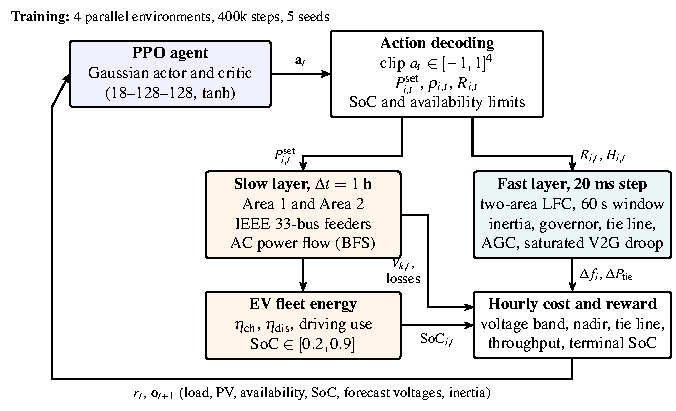
\includegraphics[width=0.78\textwidth]{fig_architecture.pdf}
\caption{Two-time-scale V2G coordination framework. The PPO agent sets
the hourly V2G set-point and the frequency-reserve share of each area.
The slow layer solves AC power flow on the IEEE 33-bus feeder of each
area and updates fleet energy; the fast layer simulates two-area LFC
dynamics with the reserve-dependent V2G droop.}
\label{fig:architecture}
\end{figure*}

\subsection{Distribution Feeders}
\label{sec:feeders}

Both areas use the branch impedances and nominal loads of the IEEE
33-bus system \cite{BaranWu1989} at 12.66~kV, taken from the pandapower
case library \cite{Thurner2018}. The five normally open tie switches are
kept open so that the feeder remains radial. The net load at bus $k$
of area $i$ in hour $t$ is
\begin{equation}
P_{k,t} = \lambda_{i,t}P_k^{0}-P^{\mathrm{PV}}_{k,t}-P^{\mathrm{EV}}_{k,t},
\qquad
Q_{k,t} = \lambda_{i,t}Q_k^{0},
\label{eq:netload}
\end{equation}
where $P_k^{0}$ and $Q_k^{0}$ are the nominal loads, $\lambda_{i,t}$ is
the normalized load profile, and positive $P^{\mathrm{EV}}_{k,t}$
denotes discharge. The fleet set-point is shared equally among the V2G
hubs of the area, and the PV output is shared equally among the PV
buses (Fig.~\ref{fig:feeder}). Area~1 is a residential feeder with
1.5~MW of PV and hubs in the downstream half of the main feeder
(buses 13, 17, and 18) and at the end of the bus 26 to 33 lateral. Area~2 is a mixed commercial and residential feeder
with 4.2~MW of PV concentrated at the feeder ends, which produces
midday overvoltage when PV output is high.

The power flow is solved by the direct backward/forward sweep of
\cite{Teng2003}. With the bus-injection to branch-current matrix
$\mathbf{B}$ and the branch impedance vector $\mathbf{z}$, the bus
voltages are updated as
\begin{equation}
\mathbf{V}^{(m+1)} = V_0\mathbf{1}-\mathbf{B}^{T}\operatorname{diag}(\mathbf{z})\mathbf{B}\,
\overline{\left(\mathbf{S}\oslash\mathbf{V}^{(m)}\right)},
\label{eq:bfs}
\end{equation}
until the largest voltage update falls below $10^{-9}$~p.u., where
$\mathbf{S}$ is the complex net load vector and $\oslash$ denotes
element-wise division. The active-power loss is
$\sum_{b}r_b|I_b|^{2}$ over all branches $b$.

\begin{figure*}[!t]
\centering
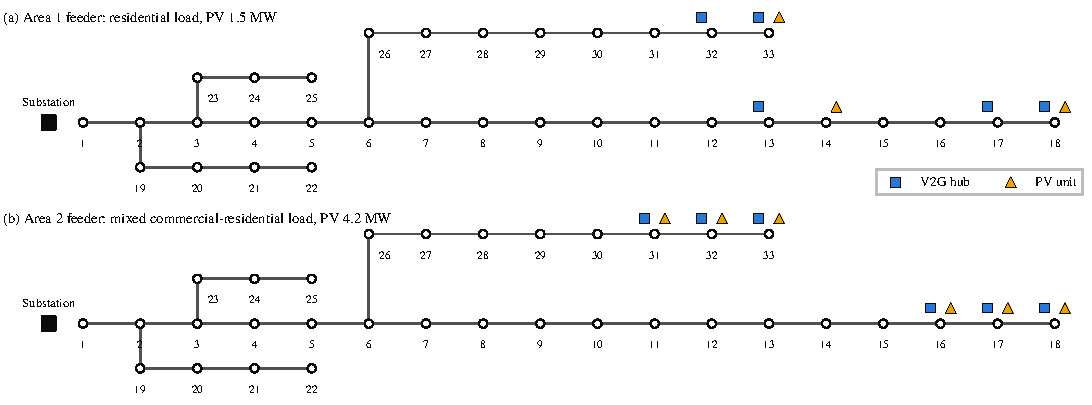
\includegraphics[width=\textwidth]{fig_feeder.pdf}
\caption{IEEE 33-bus feeders used in the two areas, with V2G hubs and
PV units. The topology and impedances are those of \cite{BaranWu1989}.}
\label{fig:feeder}
\end{figure*}

\subsection{Daily Profiles and Scenario Generation}
\label{sec:profiles}

Fig.~\ref{fig:profiles} shows the nominal daily profiles. The
residential profile has a morning shoulder and an evening peak at
19:00 to 21:00, and the mixed profile has a broad daytime plateau and an
evening peak. Both profiles are synthetic; their shapes follow the
measured residential and commercial low-voltage consumer curves of
\cite{Jardini2000}, with a residential evening peak and a commercial
daytime plateau, and are normalized to a peak of 1.0. The PV profile
follows a clear-sky shape between 06:00 and 18:00. Area~1 represents
home charging, with about 90\% of the fleet plugged in at night and 30\%
during working hours, which reproduces the pattern of residential
charging availability observed in the EV Project, low during the day
and high overnight \cite{Schey2012}. Area~2 represents workplace
charging with the opposite pattern, following the observation that
vehicles with access to workplace charging are typically parked there
for 4 to 10 h on working days \cite{INL2014}.

Each training or evaluation day is drawn from a scenario generator that
scales the area load by a factor in $[0.85,1.10]$, applies a cloud
factor in $[0.3,1.0]$ with hour-to-hour PV variability, scales fleet
participation by a factor in $[0.7,1.1]$, adds 3\% multiplicative noise
to the hourly load, and draws the initial SoC in $[0.50,0.60]$. Stress
days use heavier load ($[1.10,1.20]$), lower fleet participation
($[0.55,0.70]$), and disturbances 1.3 to 1.6 times larger, all outside
the training ranges, together with near clear-sky PV ($[0.9,1.0]$),
which lies at the upper end of the training range. Stress days are
never seen during training.

\begin{figure}[!t]
\centering
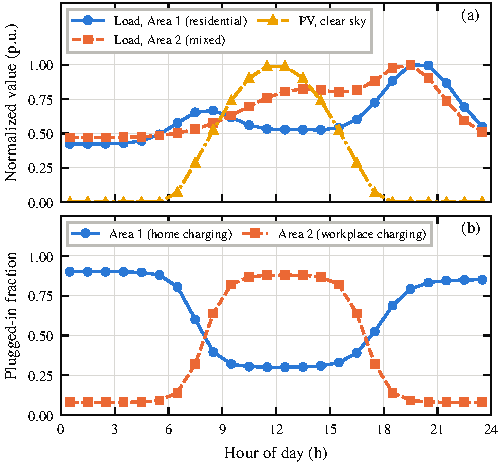
\includegraphics[width=\columnwidth]{fig_profiles.pdf}
\caption{Nominal daily profiles. (a) Normalized load of each area and
clear-sky PV. (b) Fraction of the fleet plugged in.}
\label{fig:profiles}
\end{figure}

\subsection{Aggregated EV Fleet}
\label{sec:fleet}

Each representative feeder hosts $N_{\mathrm{EV}}=300$ vehicles with
60-kWh batteries and 7.4-kW bidirectional chargers. The usable SoC
range is 0.20 to 0.90, and the charging and discharging efficiencies
are $\eta_{\mathrm{ch}}=\eta_{\mathrm{dis}}=0.92$. Each vehicle uses
9~kWh per day for driving, which corresponds to about 45~km at a
real-driving consumption of about 190~Wh/km; more than 80\% of European
drivers cover less than 65~km per day and the median real-driving
consumption of a small battery electric car was 186~Wh/km in the Green
eMotion field data \cite{Donati2015}. The driving energy is distributed
over the hours in which the vehicle is away in proportion to the
unplugged fraction. The fleet is
treated as one aggregated battery with energy capacity
$E^{\mathrm{cap}}=18$~MWh per feeder. The plugged-in rating is
\begin{equation}
P^{\mathrm{rate}}_{i,t}=\chi_{i,t}\,\kappa_i\,N_{\mathrm{EV}}\,P_{\mathrm{ch}},
\label{eq:prate}
\end{equation}
where $\chi_{i,t}$ is the plugged-in fraction and $\kappa_i$ the
participation factor of the scenario. With the driving energy
$E^{\mathrm{drv}}_{i,t}$ deducted first, the energy-feasible limits
for $\Delta t=1$~h are
\begin{align}
\bar P^{\mathrm{dis}}_{i,t}&=\min\!\left\{P^{\mathrm{rate}}_{i,t},\,
\eta_{\mathrm{dis}}\frac{E_{i,t}-E^{\mathrm{drv}}_{i,t}-E^{\min}}{\Delta t}\right\}^{+},
\label{eq:pdis}\\
\bar P^{\mathrm{ch}}_{i,t}&=\min\!\left\{P^{\mathrm{rate}}_{i,t},\,
\frac{E^{\max}-E_{i,t}+E^{\mathrm{drv}}_{i,t}}{\eta_{\mathrm{ch}}\Delta t}\right\}^{+},
\label{eq:pch}
\end{align}
and the energy is updated as
\begin{equation}
E_{i,t+1}=E_{i,t}-\frac{P^{\mathrm{dis}}_{i,t}\Delta t}{\eta_{\mathrm{dis}}}
+\eta_{\mathrm{ch}}P^{\mathrm{ch}}_{i,t}\Delta t-E^{\mathrm{drv}}_{i,t}
+\Delta E^{\mathrm{reg}}_{i,t},
\label{eq:energy}
\end{equation}
with $P^{\mathrm{dis}}=\max(P^{\mathrm{set}},0)$ and
$P^{\mathrm{ch}}=\max(-P^{\mathrm{set}},0)$. If driving alone would take
the energy below $E^{\min}$, the shortfall is recorded as unmet
mobility energy and penalized.

The last term of \eqref{eq:energy} is the battery energy exchanged by
the frequency droop loop of Section~\ref{sec:lfcmodel}. The fast layer
simulates a window of length $\tau_w=60$~s in every hour, which is
too short to integrate the energy of a full hour directly. Four
treatments of this term are compared in Section~\ref{sec:regenergy}.
Let $E^{\mathrm{out}}$ and $E^{\mathrm{in}}$ denote the energy
delivered to and absorbed from the grid by the area droop power over a
simulated interval, $E^{\mathrm{out}}=\int\max(\Delta P_{\mathrm{ev},i},0)\,d\tau$
and $E^{\mathrm{in}}=\int\max(-\Delta P_{\mathrm{ev},i},0)\,d\tau$. The
battery-side energy per feeder is
\begin{equation}
\Delta E^{\mathrm{reg}}_{i,t}=\frac{1}{N_f}\left(
-\frac{E^{\mathrm{out}}_{i,t}}{\eta_{\mathrm{dis}}}+\eta_{\mathrm{ch}}E^{\mathrm{in}}_{i,t}\right),
\label{eq:regenergy}
\end{equation}
so that every round trip is lossy. The treatments differ in how
$E^{\mathrm{out}}$ and $E^{\mathrm{in}}$ are obtained for the hour:
(i) \emph{none}, the term is neglected (the model of the first
submission, used for diagnosis only); (ii) \emph{window}, only the
simulated 60~s are counted; (iii) \emph{hourly extrapolation}, the
window energy is multiplied by $3600/\tau_w=60$, which implicitly
assumes that the step disturbance of the window recurs every minute;
(iv) \emph{decomposed}, the window containing the step event is counted
once and a second 60-s simulation of the same hour with the
fluctuating component only is scaled to the remaining 59~min,
\begin{equation}
E^{\mathrm{out}}_{i,t}=E^{\mathrm{out}}_{\mathrm{step+fluct}}
+\left(\frac{3600}{\tau_w}-1\right)E^{\mathrm{out}}_{\mathrm{fluct}},
\label{eq:decomposed}
\end{equation}
and likewise for $E^{\mathrm{in}}$. Treatment (iv) is the default of the
environment used for training and for all reported results. Its
accuracy is checked against an exact 3600-s simulation of the fast
layer for every hour of the evaluation (Section~\ref{sec:regenergy}),
which is too slow to use during training.

\subsection{Two-Area Load-Frequency Control Model}
\label{sec:lfcmodel}

The fast layer uses the standard linearized two-area LFC model
\cite{Kundur1994,Bevrani2014} with non-reheat turbines, extended with a
V2G droop loop in each area \cite{Izadkhast2015}. In per unit on the
area base $P_r=500$~MW and with frequency deviation $\Delta f_i$ in per
unit of $f_0=50$~Hz,
\begin{align}
2H_{i,t}\,\dot{\Delta f_i}&=\Delta P_{m,i}+\Delta P_{\mathrm{ev},i}-\Delta P_{L,i}
-a_i\Delta P_{\mathrm{tie}}-D_i\Delta f_i,\label{eq:swing}\\
T_{g,i}\,\dot{\Delta P_{g,i}}&=\Delta P_{c,i}-\Delta f_i/R_i-\Delta P_{g,i},\\
T_{t,i}\,\dot{\Delta P_{m,i}}&=\Delta P_{g,i}-\Delta P_{m,i},\\
\dot{\Delta P_{\mathrm{tie}}}&=2\pi f_0T_{12}\,(\Delta f_1-\Delta f_2),\\
\mathrm{ACE}_i&=B_i\Delta f_i+a_i\Delta P_{\mathrm{tie}},\quad
\Delta P_{c,i}=-K_I\!\int\!\mathrm{ACE}_i\,dt,\label{eq:ace}\\
T_{\mathrm{ev}}\,\dot{\Delta P_{\mathrm{ev},i}}&=
\operatorname{sat}_{\pm r_{i,t}}\!\left(-K_{\mathrm{ev},i,t}\Delta f_i\right)-\Delta P_{\mathrm{ev},i},
\label{eq:evdroop}
\end{align}
where $a_1=1$, $a_2=-1$, $B_i=1/R_i+D_i$, and $r_{i,t}=N_fR_{i,t}/P_r$
is the area V2G reserve in per unit. The droop gain is
$K_{\mathrm{ev},i,t}=r_{i,t}f_0/\Delta f_{\mathrm{full}}$, so the full
reserve is deployed at $\Delta f_{\mathrm{full}}=0.2$~Hz and the
response saturates beyond that point. The first-order lag
$T_{\mathrm{ev}}=0.15$~s represents aggregator communication and
converter response. Aggregated EV fleets are commonly represented in
LFC studies by a first-order transfer function with time constants
between 0.1 and 1~s \cite{KoSung2018,Ziras2017}; the chosen value lies
at the fast end of this range; the settling time of about 1~s
measured for charger response to local frequency measurements and
reported in \cite{Ziras2017} corresponds to roughly three to five such
time constants.

Inertia falls when PV displaces synchronous generation. The hourly
inertia constant is
\begin{equation}
H_{i,t}=H_i^{0}\left(1-\gamma_i S_{i,t}\right),
\label{eq:inertia}
\end{equation}
where $S_{i,t}$ is the normalized PV output and $\gamma_1=0.20$,
$\gamma_2=0.35$ reflect the higher PV share of Area~2
\cite{Tielens2016}. In each hour the window contains a step load change
at $t=2$~s in one randomly selected area, with magnitude
$0.03\,\delta\,u$~p.u., where $\delta$ is the scenario disturbance scale
and $u$ is uniform in $[0.5,1.0]$ with a random sign, plus an
Ornstein--Uhlenbeck fluctuation with a 10-s time constant and standard
deviation $0.006\,(0.3+2S_{i,t}(1.2-c_i))$~p.u., where $c_i$ is the
cloud factor, so that the fluctuation grows with PV output under
partial cloud. The disturbance of
each hour is generated from a seed fixed by the scenario and the hour,
so every controller faces identical disturbances. Equations
\eqref{eq:swing} to \eqref{eq:evdroop} are integrated with the
fourth-order Runge--Kutta method. Table~\ref{tab:params} lists all
parameters.

\begin{table}[!t]
\caption{Model, fleet, and training parameters.}
\label{tab:params}
\centering
\footnotesize
\setlength{\tabcolsep}{3pt}
\begin{tabular}{p{0.60\columnwidth}p{0.34\columnwidth}}
\toprule
\textbf{Parameter} & \textbf{Value}\\
\midrule
\multicolumn{2}{l}{\emph{Feeder and fleet (per representative feeder)}}\\
Feeder / base voltage & IEEE 33-bus / 12.66 kV\\
PV rating, Area 1 / Area 2 & 1.5 / 4.2 MW\\
EVs, battery, charger & 300, 60 kWh, 7.4 kW\\
SoC limits; $\eta_{\mathrm{ch}}=\eta_{\mathrm{dis}}$ & 0.20 to 0.90; 0.92\\
Driving energy per EV & 9 kWh/day\\
Feeders per area $N_f$ & 25\\
\multicolumn{2}{l}{\emph{Two-area LFC}}\\
Area base $P_r$; $f_0$ & 500 MW; 50 Hz\\
$H_1^0$, $H_2^0$; $\gamma_1$, $\gamma_2$ & 5.0, 4.0 s; 0.20, 0.35\\
$D_i$; $R_i$ & 1.0 p.u.; 0.05 p.u.\\
$T_{g,1}$, $T_{g,2}$; $T_{t,1}$, $T_{t,2}$ & 0.08, 0.10 s; 0.40, 0.45 s\\
$T_{12}$; $K_I$ & 0.08 p.u./rad; 0.05\\
$T_{\mathrm{ev}}$; $\Delta f_{\mathrm{full}}$ & 0.15 s; 0.2 Hz\\
Window; integration step & 60 s; 20 ms (RK4)\\
Load step; OU base std. & 0.03$\delta u$; 0.006 p.u.\\
\multicolumn{2}{l}{\emph{Control and reward}}\\
Voltage band & 0.95 to 1.05 p.u.\\
$\rho_{\max}$ & 0.6\\
$w_V$, $w_f$, $w_{\mathrm{tie}}$, $w_{\mathrm{deg}}$, $w_E$, $w_U$ & 50, 4, 0.5, 0.05, 1, 100\\
\multicolumn{2}{l}{\emph{PPO}}\\
Actor and critic & 18--128--128, tanh\\
Learning rate & $3\times10^{-4}$, linear decay to 0\\
Rollout; minibatch; epochs & $4\times384$; 256; 10\\
Initial $\log\sigma$; entropy coef. & $-0.5$; 0\\
$\gamma$; GAE $\lambda$; clip $\epsilon$ & 0.995; 0.95; 0.2\\
Training steps; seeds & 400\,000; 5\\
\bottomrule
\end{tabular}
\end{table}

% ============================================================
\section{Control Problem and Learning Procedure}
\label{sec:control}
% ============================================================

\subsection{Observation and Action}
\label{sec:obsact}

At the start of hour $t$ the agent observes
\begin{multline}
\mathbf{o}_t=\Big[\sin\theta_t,\cos\theta_t,\lambda_{1,t},\lambda_{2,t},
S_{1,t},S_{2,t},\chi_{1,t}\kappa_1,\chi_{2,t}\kappa_2,\\
\widetilde{\mathrm{SoC}}_{1,t},\widetilde{\mathrm{SoC}}_{2,t},
\tilde V^{0}_{\cdot,t},\frac{H_{1,t}}{H_1^0},\frac{H_{2,t}}{H_2^0},\delta,\tau_t\Big],
\label{eq:obs}
\end{multline}
where $\theta_t$ encodes the hour of day, $\tilde V^{0}_{\cdot,t}$ are
the normalized minimum and maximum feeder voltages of both areas
forecast for zero fleet power (four entries), and $\tau_t$ is the
remaining fraction of the horizon, for 18 entries in total. The load,
PV, and availability entries are treated as hour-ahead forecasts; the
disturbance realization of the hour is not observed.

The action $\mathbf{a}_t\in\mathbb{R}^4$ sampled from the Gaussian
policy is clipped to $[-1,1]^4$ before it is applied. The first two
entries set the normalized set-points and the last two the reserve
shares,
\begin{align}
\rho_{i,t}&=\rho_{\max}\frac{a_{i+2,t}+1}{2},\nonumber\\
P^{\mathrm{set}}_{i,t}&=\Pi_{[-\bar P^{\mathrm{ch}}_{i,t},\,\bar P^{\mathrm{dis}}_{i,t}]}
\left(a_{i,t}(1-\rho_{i,t})P^{\mathrm{rate}}_{i,t}\right),
\label{eq:decode}
\end{align}
where $\Pi$ denotes projection onto the interval. Two limiting
operations are recorded separately. A raw-action clipping is counted
for every component of the Gaussian action that lies outside
$[-1,1]$ before clipping; because the training library clips actions
before they reach the environment, this count is obtained in
evaluation from the unclipped mean of the policy. A projection event
is counted when the projection $\Pi$ in \eqref{eq:decode} is active,
that is, when a set-point within the action range is not physically
feasible. The reserve that the fleet can deliver symmetrically around
the set-point is
\begin{equation}
R_{i,t}=\min\left\{\rho_{i,t}P^{\mathrm{rate}}_{i,t},\;
P^{\mathrm{rate}}_{i,t}-|P^{\mathrm{set}}_{i,t}|,\;
R^{\uparrow}_{i,t},\;R^{\downarrow}_{i,t}\right\}^{+},
\label{eq:reserve}
\end{equation}
where the first two terms are the requested share and the converter
headroom, and $R^{\uparrow}$ and $R^{\downarrow}$ are the largest
upward and downward activations that, sustained for the whole hour,
keep the stored energy inside $[E^{\min},E^{\max}]$. With the energy
after the schedule
$E^{\mathrm{s}}_{i,t}=E_{i,t}-E^{\mathrm{drv}}_{i,t}
-P^{\mathrm{dis}}_{i,t}\Delta t/\eta_{\mathrm{dis}}
+\eta_{\mathrm{ch}}P^{\mathrm{ch}}_{i,t}\Delta t$,
the room above the floor $A=E^{\mathrm{s}}_{i,t}-E^{\min}$, and the room
below the ceiling $B=E^{\max}-E^{\mathrm{s}}_{i,t}$,
\begin{align}
R^{\uparrow}_{i,t}&=
\begin{cases}
0, & A\le 0,\\
A/(\eta_{\mathrm{ch}}\Delta t), & 0<A\le\eta_{\mathrm{ch}}P^{\mathrm{ch}}_{i,t}\Delta t,\\
P^{\mathrm{ch}}_{i,t}+\eta_{\mathrm{dis}}\!\left(\dfrac{A}{\Delta t}-\eta_{\mathrm{ch}}P^{\mathrm{ch}}_{i,t}\right), & \text{otherwise},
\end{cases}\label{eq:rup}\\
R^{\downarrow}_{i,t}&=
\begin{cases}
0, & B\le 0,\\
\eta_{\mathrm{dis}}B/\Delta t, & 0<B\le \dfrac{P^{\mathrm{dis}}_{i,t}\Delta t}{\eta_{\mathrm{dis}}},\\[4pt]
P^{\mathrm{dis}}_{i,t}+\dfrac{B/\Delta t-P^{\mathrm{dis}}_{i,t}/\eta_{\mathrm{dis}}}{\eta_{\mathrm{ch}}}, & \text{otherwise}.
\end{cases}\label{eq:rdn}
\end{align}
Equation~\eqref{eq:rup} accounts for the two paths of an upward
activation: reducing a scheduled charging power saves
$\eta_{\mathrm{ch}}$ megawatt-hours of stored energy per megawatt-hour
of activation, whereas activation beyond the charging power becomes a
discharge that costs $1/\eta_{\mathrm{dis}}$. Equation~\eqref{eq:rdn}
is the mirror image for a downward activation. When driving alone
takes the fleet below $E^{\min}$ ($A\le0$), no upward reserve is
credited, because the charging needed to cover the mobility shortfall
cannot be given up. Equations \eqref{eq:decode} to \eqref{eq:rdn}
guarantee that the set-point plus the droop power stays within the
charger rating at every instant and that a full activation of
$R_{i,t}$ in either direction, sustained for the whole hour, keeps the
energy within its limits. Both properties are verified numerically in
Section~\ref{sec:regenergy}; the second is a design guarantee that does
not depend on the length of the simulated window.

\subsection{Reward}
\label{sec:reward}

The hourly reward is $r_t=-0.1\,c_t$ with
\begin{align}
c_t={}&w_V\sum_{i=1}^{2}\sum_{k=2}^{33}\Big[(0.95-V_{k,t}^{(i)})^{+}
+w_{\mathrm{ov}}(V_{k,t}^{(i)}-1.05)^{+}\Big]\nonumber\\
&+w_f\sum_{i=1}^{2}\frac{\max_\tau|\Delta f_i(\tau)|}{0.1~\mathrm{Hz}}
+w_{\mathrm{tie}}\frac{\mathrm{RMS}(\Delta P_{\mathrm{tie}})}{10~\mathrm{MW}}\nonumber\\
&+w_{\mathrm{deg}}\sum_{i=1}^{2}\frac{100|P^{\mathrm{set}}_{i,t}|\Delta t}{E^{\mathrm{cap}}}
+w_U\sum_{i=1}^{2}\frac{E^{\mathrm{unmet}}_{i,t}}{E^{\mathrm{cap}}}\nonumber\\
&+\mathbb{1}_{t=23}\,w_E\sum_{i=1}^{2}100\left(\mathrm{SoC}_{i,0}-\mathrm{SoC}_{i,24}\right)^{+}.
\label{eq:cost}
\end{align}
The voltage term penalizes both undervoltage and overvoltage with
$w_{\mathrm{ov}}=1$. The frequency term uses the nadir of each area,
normalized by 0.1~Hz, and the tie-line term uses the RMS deviation
normalized by 10~MW. The throughput term is a linear proxy for battery
wear expressed in percent of capacity per hour; energy throughput has
been identified as the dominant driver of degradation for EV batteries
providing V2G services \cite{Bishop2013}. The terminal term
penalizes each percentage point of SoC deficit at the end of the day,
so that the fleet returns to at least its initial energy. The weights
were chosen so that a typical uncontrolled day produces voltage and
frequency costs of the same order of magnitude; Section~\ref{sec:ablation}
reports the effect of removing individual terms.

\subsection{PPO Training}
\label{sec:ppo}

The agent is trained with the PPO implementation of Stable-Baselines3
\cite{Raffin2021} using the clipped surrogate objective
\cite{Schulman2017} and generalized advantage estimation \cite{Schulman2016}.
Four environments run in parallel, each drawing a new random day at
reset, and the hyperparameters are those of Table~\ref{tab:params}.
Every 6144 environment steps, the deterministic policy (the mean of the
Gaussian) is evaluated on ten fixed validation days that are disjoint
from the training stream and from the test sets, and the parameters
with the best validation return are retained. Training is considered
converged when the validation return changes by less than 2\% over the
final 50\,000 steps. Five independent seeds (0 to 4) are trained, and
all results are reported across seeds, as recommended for RL
benchmarks \cite{Henderson2018}. All policies reported in this paper,
including the ablation and sensitivity variants, were trained from
scratch in the final version of the environment described above; no
checkpoint from an earlier model version is used.

The Gaussian policy of PPO is unbounded and the library clips sampled
actions to the action box before they reach the environment. As a
bounded-action alternative, a policy with a hyperbolic-tangent squashed
output and generalized state-dependent exploration \cite{Raffin2022}
is trained with the same budget as the ablation reference and compared
in Section~\ref{sec:clip}.

\subsection{Benchmark Controllers}
\label{sec:bench}

All benchmarks run in the same environment, with the same scenarios,
disturbances, network, and constraints as PPO, and are evaluated with
the same cost \eqref{eq:cost}.

\emph{Uncontrolled charging (UC):} plugged-in vehicles charge at the
full available rate until $\mathrm{SoC}_{\max}$ is reached, with no V2G
discharge and no frequency reserve.

\emph{Rule-based control (RB):} a conventional local controller. The
set-point follows a volt-watt characteristic on the forecast feeder
voltages, rising linearly from zero at $V_{\min}=0.965$~p.u. to full
discharge at 0.94~p.u. and falling to full charge as $V_{\max}$ rises
from 1.035 to 1.05~p.u. When no voltage action is required and the SoC
is below its initial value plus 0.1, the fleet charges at full rate
during 00:00 to 06:00 (and during 09:00 to 15:00 in Area~2). Discharge
is blocked below SoC 0.40, and a fixed reserve share $\rho=0.3$ is
held for frequency droop.

\emph{Day-ahead optimization (DAO):} with perfect foresight of load,
PV, and availability, the 24 hourly set-points of each area are
optimized by Powell's method with the AC power flow and the fleet
energy model inside the objective, minimizing the voltage, throughput,
unmet-energy, and terminal-SoC terms of \eqref{eq:cost}. The reserve
share is fixed at $\rho=0.3$. The search starts from an open-loop
volt-watt schedule with fixed night-time (and, in Area~2, PV-hour)
charging and is limited to 20 Powell iterations; on the days checked,
raising the limit to 80 iterations did not change the solution, but
the method is local and the schedule is not guaranteed to be globally
optimal. DAO serves as an informed benchmark for the voltage and
energy part of the problem; it does not optimize the reserve
allocation.

\subsection{Evaluation Protocol and Metrics}
\label{sec:protocol}

The test set contains 30 days drawn from the training distribution with
an independent random stream, and the stress set contains 20
out-of-distribution days as defined above. For each controller and day
the following daily metrics are computed: hours with any bus outside
0.95 to 1.05~p.u. (summed over the two areas); integrated undervoltage
and overvoltage in p.u.$\cdot$h summed over all buses; the daily
minimum and maximum voltages; the mean over hours of the larger area
frequency nadir; the worst nadir; the RMS frequency deviation; the
maximum rate of change of frequency (RoCoF) over a 500-ms window; the
RMS tie-line deviation; the area-level fleet throughput; the SoC
deficit at the end of the day; unmet mobility energy; the battery-side
regulation energy \eqref{eq:regenergy} under each treatment, including
the exact 3600-s simulation; the numbers of raw-action clippings per
action dimension and of projection events; the largest excess of the
scheduled plus droop power over the charger and energy limits; the
smallest sustained-activation energy margin; any SoC-limit violation;
and the feeder energy loss. PPO results are pooled over the five seeds and the
days, and seed-to-seed variability is reported separately as the
standard deviation of the per-seed means.

% ============================================================
\section{Results and Discussion}
\label{sec:results}
% ============================================================

\subsection{Model Verification}
\label{sec:verif}

The backward/forward sweep reproduces the published base case of the
IEEE 33-bus feeder: the minimum voltage is \ValVmin~p.u.\ at bus 18 and
the active-power loss is \ValLoss~kW, in agreement with
\cite{BaranWu1989}. Over 20 random operating points with load factors
between 0.4 and 1.1 and five random injections of up to $\pm0.8$~MW,
the largest voltage difference from the Newton--Raphson solution of
pandapower \cite{Thurner2018} is $\ValVerr$~p.u. For the LFC model with
AGC disabled, a 0.02-p.u.\ step in Area~1 gives a steady-state frequency
deviation of \ValDfSim~Hz and a tie-line change of \ValTieSim~MW, equal
to the closed-form values $-\Delta P_L f_0/(B_1+B_2)=\ValDfTh$~Hz and
$-\Delta P_LB_2P_r/(B_1+B_2)=\ValTieTh$~MW. With AGC active, both
quantities return to zero, and the inter-area mode lies near
\ValMode~Hz. The verification scripts are part of the released code.

\subsection{Training Behavior}
\label{sec:training}

Fig.~\ref{fig:learning} shows the daily cost on the training episodes
and on the ten validation days for the \NSeed{} seeds. Every seed is below
the validation cost of the rule-based controller at the second
evaluation (6144 steps) and falls below that of the day-ahead
optimization between \CrossDAOLo{} and \CrossDAOHi{} steps. Over the
final 50\,000 steps, the validation cost of every seed changes by at
most \ConvChangePct\%, which satisfies the convergence criterion of
Section~\ref{sec:control}. The final validation cost is
\FinalValCost~$\pm$~\FinalValCostSd{} across seeds, compared with
\ValDAO{} for DAO, \ValRB{} for RB, and \ValUC{} for UC on the same
days. The narrow seed-to-seed spread indicates that the result does not
depend on a favorable initialization. Training one seed takes about
\TrainMin~min on a single CPU core.

\begin{figure}[!t]
\centering
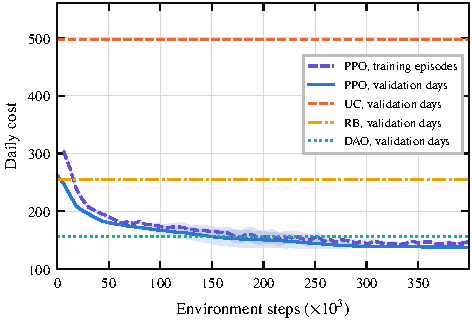
\includegraphics[width=\columnwidth]{fig_learning.pdf}
\caption{PPO learning curves (mean and $\pm1$ standard deviation over
\NSeed{} seeds) on training episodes and on ten fixed validation days,
with the benchmark costs on the validation days.}
\label{fig:learning}
\end{figure}

\subsection{Performance on Held-Out Test Days}
\label{sec:testres}

Table~\ref{tab:test} summarizes the 30 test days. PPO attains a mean
daily cost of \TPPOCost, which is \TRedCostDAO\% lower than DAO,
\TRedCostRB\% lower than RB, and \TRedCostUC\% lower than UC. The
seed-averaged PPO cost is lower than that of DAO on \TWinsDAO{} of the
30 days and lower than that of RB and UC on \TWinsRB{} and \TWinsUC{}
days, respectively, and the paired Wilcoxon signed-rank test on the seed-averaged
daily costs gives $p=\TPDAO$ against each benchmark.

\begin{table*}[!t]
\caption{Results on the 30 held-out test days (mean $\pm$ standard deviation across days). PPO values are pooled over 5 seeds; the value in parentheses is the standard deviation of the per-seed means.}
\label{tab:test}
\centering
\footnotesize
\begin{tabular}{lcccc}
\toprule
\textbf{Metric} & \textbf{UC} & \textbf{RB} & \textbf{DAO} & \textbf{PPO (proposed)}\\
\midrule
Daily cost $\sum_t c_t$ & 477.2 $\pm$ 74.8 & 245.5 $\pm$ 31.6 & 152.3 $\pm$ 31.8 & 135.5 $\pm$ 26.0 (1.3) \\
Voltage-violation hours (h) & 19.3 $\pm$ 3.4 & 12.5 $\pm$ 2.1 & 18.2 $\pm$ 4.0 & 11.9 $\pm$ 5.5 (1.1) \\
Undervoltage (p.u.$\cdot$h) & 7.40 $\pm$ 1.49 & 2.86 $\pm$ 0.59 & 1.04 $\pm$ 0.37 & 0.90 $\pm$ 0.35 (0.01) \\
Overvoltage (p.u.$\cdot$h) & 0.050 $\pm$ 0.082 & 0.001 $\pm$ 0.005 & 0.001 $\pm$ 0.005 & 0.004 $\pm$ 0.016 (0.001) \\
Minimum voltage (p.u.) & 0.835 $\pm$ 0.015 & 0.907 $\pm$ 0.007 & 0.922 $\pm$ 0.007 & 0.925 $\pm$ 0.006 (0.000) \\
Maximum voltage (p.u.) & 1.044 $\pm$ 0.028 & 1.024 $\pm$ 0.016 & 1.029 $\pm$ 0.019 & 1.024 $\pm$ 0.022 (0.000) \\
Mean hourly nadir (mHz) & 54.4 $\pm$ 6.2 & 49.4 $\pm$ 6.0 & 49.8 $\pm$ 6.0 & 47.3 $\pm$ 5.9 (0.1) \\
Worst nadir (mHz) & 79.2 $\pm$ 10.4 & 70.5 $\pm$ 7.6 & 70.5 $\pm$ 7.6 & 69.6 $\pm$ 7.5 (0.4) \\
RMS frequency deviation (mHz) & 12.80 $\pm$ 1.22 & 11.48 $\pm$ 1.16 & 11.57 $\pm$ 1.18 & 10.87 $\pm$ 1.10 (0.01) \\
Maximum RoCoF (Hz/s) & 0.154 $\pm$ 0.024 & 0.137 $\pm$ 0.016 & 0.137 $\pm$ 0.016 & 0.133 $\pm$ 0.015 (0.001) \\
RMS tie-line deviation (MW) & 2.51 $\pm$ 0.23 & 2.49 $\pm$ 0.24 & 2.49 $\pm$ 0.24 & 2.51 $\pm$ 0.25 (0.00) \\
Mean V2G reserve, both areas (MW) & 0.0 $\pm$ 0.0 & 15.2 $\pm$ 1.4 & 13.9 $\pm$ 2.6 & 25.3 $\pm$ 2.8 (0.3) \\
Fleet throughput, area level (MWh) & 491 $\pm$ 19 & 337 $\pm$ 92 & 348 $\pm$ 26 & 446 $\pm$ 39 (3) \\
Terminal SoC deficit (\%) & 0.00 $\pm$ 0.00 & 13.58 $\pm$ 14.06 & 9.68 $\pm$ 13.55 & 6.31 $\pm$ 6.80 (0.69) \\
Projection events per day & 27.8 $\pm$ 5.0 & 0.0 $\pm$ 0.0 & 1.6 $\pm$ 2.8 & 0.0 $\pm$ 0.0 (0.0) \\
Energy loss, two feeders (MWh) & 4.978 $\pm$ 0.595 & 3.416 $\pm$ 0.261 & 3.217 $\pm$ 0.338 & 3.159 $\pm$ 0.357 (0.015) \\
Unmet mobility energy (MWh) & 0.00 $\pm$ 0.00 & 0.00 $\pm$ 0.00 & 1.28 $\pm$ 2.55 & 0.00 $\pm$ 0.00 (0.00) \\
\bottomrule
\end{tabular}
\end{table*}


\emph{Voltage.} Uncontrolled charging coincides with the residential
evening peak and drives the Area~1 voltage down to \TUCVminDay~p.u.\ on
average, with \TUCUvPuH~p.u.$\cdot$h of integrated undervoltage per
day. PPO reduces the undervoltage to \TPPOUvPuH~p.u.$\cdot$h, which is
\TRedUvPuHUC\% below UC, \TRedUvPuHRB\% below RB, and \TRedUvPuHDAO\%
below DAO, and it lowers the number of violation hours from
\TDAOViolHours{} with DAO to \TPPOViolHours. Most of the remaining
violation hours are shallow (a few thousandths of a per unit) on the
Area~1 feeder. Deeper violations remain in Area~2 between 18:00 and
21:00, when only a small part of the workplace fleet is still plugged
in (Fig.~\ref{fig:heatmap}). Overvoltage is rare for all
controllers on the test days because the Area~2 workplace fleet
absorbs midday PV; the PPO maximum voltage is \TPPOVmaxDay~p.u.

\emph{Frequency.} PPO holds an average of \TPPOReserveMeanMw~MW of V2G
reserve across both areas, against \TRBReserveMeanMw~MW for RB and \TDAOReserveMeanMw~MW for DAO,
which hold a fixed 30\% share. The mean hourly nadir falls from
\TUCNadirMeanHz~mHz with UC to \TPPONadirMeanHz~mHz, and it is
\TRedNadirMeanHzDAO\% lower than with DAO. The maximum RoCoF decreases
by \TRedRocofMaxUC\% relative to UC. These gains are modest in absolute
terms because the V2G reserve is a small fraction of the 500-MW area
base and the governors respond within about one second. They are
nonetheless obtained without degrading the voltage objective, which is
the point of the joint allocation.

\emph{Energy and fleet.} PPO leaves a terminal SoC deficit of
\TPPOSocDefPct\%, against \TDAOSocDefPct\% for DAO and \TRBSocDefPct\%
for RB. Its fleet throughput, \TPPOThroughputMwh~MWh at area level, is
higher than that of DAO (\TDAOThroughputMwh~MWh) and RB because the
policy charges during the day to supply the evening discharge.
Section~\ref{sec:regenergy} examines the energy and power limits in
detail.

\subsection{Regulation Energy, Treatment Sensitivity, and Feasibility Audit}
\label{sec:regenergy}

\emph{Physical interpretation of the hourly extrapolation.} The 60-s
window of each hour contains one step load change at $t=2$~s and a
continuous fluctuation. Multiplying the window energy by 60 therefore
assumes that the step event recurs every minute, whereas the model
defines one step per hour. The exact 3600-s simulations recorded for
every evaluated hour show how large the error is. For the PPO
policies the gross regulation energy over the test days is
\TrkPPOGrossFull~MWh per day in the exact simulation, against
\TrkPPOGrossHour~MWh with the hourly extrapolation
(\TrkPPOGrossHourRatio{} times too large) and \TrkPPOGrossWin~MWh with
the window alone (more than 20 times too small). The decomposed
treatment \eqref{eq:decomposed} gives \TrkPPOGrossDec~MWh, or
\TrkPPOGrossDecRatio{} of the exact value. The same ratio of
\TrkRBGrossDecRatio{} to \TrkDAOGrossDecRatio{} is found for RB and
DAO, so the remaining 6\% shortfall is systematic rather than random.
A likely cause, which we state as an interpretation, is that the
fluctuation-only window starts from rest, so that its first seconds
under-represent the stationary fluctuation before the scaling to 59
minutes. The net daily energies are
\TrkPPONetFull~MWh (exact), \TrkPPONetDec~MWh (decomposed),
\TrkPPONetHour~MWh (hourly extrapolation), and \TrkPPONetWin~MWh
(window). The hourly extrapolation also gets the sign of the hourly
net energy wrong in \TrkPPOSignFlipPct\% of the hours, because the sign
of the single step event dominates the window while the full hour is
dominated by the fluctuation and by the lossy round trips. The same
ratios are found for RB and DAO (gross ratio \TrkRBGrossHourRatio{} and
\TrkDAOGrossHourRatio{} for the extrapolation, \TrkRBGrossDecRatio{}
and \TrkDAOGrossDecRatio{} for the decomposition). Repeating the 60-s
response for an entire hour is therefore not a physically justified
treatment: it overstates both the gross and the net regulation energy
by a factor of about two to three, and it is not simply conservative,
because its error has either sign hour by hour. The decomposed
treatment is closer to the exact simulation than any other cheap
treatment but underestimates the gross energy by about 6\%.

\emph{Sensitivity of the results to the treatment.}
Table~\ref{tab:modes} evaluates every controller on the same 30 test
days under the five treatments. For PPO, the daily cost changes by at
most \ModeDeltaCostHour{} between any treatment and the default, which
is \ModeDeltaCostSdHour{} times the seed-to-seed standard deviation of
the final policies (\PPOSeedSd); the undervoltage and the violation hours change by at
most 0.001~p.u.$\cdot$h and 0.1~h, the nadir is unchanged to the
reported precision, and the terminal SoC deficit moves between
\ModeNonePPOSocDefPct\% (neglected) and \ModeHourPPOSocDefPct\%
(hourly extrapolation). No treatment produces an SoC-limit violation
or any additional unmet mobility energy for any controller; the unmet
energy of DAO (\ModeDecomposedDAOUnmetMwh~MWh) is caused by its
schedule and is the same under all treatments to within 0.03~MWh. The regulation-energy assumption therefore does not change
the control problem, the ranking of the controllers, or any
conclusion of this paper. The decomposed treatment is retained as the
default because it tracks the exact simulation to within 6\% at the
cost of one additional 60-s simulation per hour.

\begin{table*}[!t]
\caption{Sensitivity of the daily results on the 30 test days to the treatment of the regulation energy. Every row uses the same scenarios, disturbances and controllers; only the energy credited to the droop loop in \eqref{eq:energy} differs. PPO rows pool the five final policies. The last column is the energy by which the stored energy would have left $[E^{\min},E^{\max}]$ without the limit.}
\label{tab:modes}
\centering
\scriptsize
\setlength{\tabcolsep}{3pt}
\begin{tabular}{llcccccccc}
\toprule
\textbf{Controller} & \textbf{Treatment} & \textbf{Cost} & \textbf{SoC def. (\%)} & \textbf{Unmet (MWh)} & \textbf{UV (p.u.$\cdot$h)} & \textbf{Viol. h} & \textbf{Nadir (mHz)} & \textbf{Reg. energy (MWh/d)} & \textbf{Limit viol. (MWh)}\\
\midrule
\multirow{5}{*}{UC} & None (neglected) & 477.2 & 0.00 & 0.00 & 7.402 & 19.3 & 54.4 & 0.00 & 0.000 \\
& 60-s window only & 477.2 & 0.00 & 0.00 & 7.402 & 19.3 & 54.4 & 0.00 & 0.000 \\
& Hourly extrapolation ($\times 60$) & 477.2 & 0.00 & 0.00 & 7.402 & 19.3 & 54.4 & 0.00 & 0.000 \\
& Decomposed (default) & 477.2 & 0.00 & 0.00 & 7.402 & 19.3 & 54.4 & 0.00 & 0.000 \\
& Exact 3600-s simulation & 477.2 & 0.00 & 0.00 & 7.402 & 19.3 & 54.4 & 0.00 & 0.000 \\
\midrule
\multirow{5}{*}{RB} & None (neglected) & 245.0 & 13.71 & 0.00 & 2.848 & 12.5 & 49.4 & 0.00 & 0.000 \\
& 60-s window only & 245.0 & 13.72 & 0.00 & 2.848 & 12.5 & 49.4 & -0.02 & 0.000 \\
& Hourly extrapolation ($\times 60$) & 247.0 & 13.66 & 0.00 & 2.887 & 12.6 & 49.4 & -1.10 & 0.000 \\
& Decomposed (default) & 245.5 & 13.58 & 0.00 & 2.860 & 12.5 & 49.4 & -0.46 & 0.000 \\
& Exact 3600-s simulation & 245.1 & 13.75 & 0.00 & 2.848 & 12.5 & 49.4 & -0.50 & 0.000 \\
\midrule
\multirow{5}{*}{DAO} & None (neglected) & 152.2 & 9.59 & 1.28 & 1.045 & 18.2 & 49.8 & 0.00 & 0.000 \\
& 60-s window only & 152.2 & 9.59 & 1.28 & 1.045 & 18.2 & 49.8 & -0.02 & 0.000 \\
& Hourly extrapolation ($\times 60$) & 152.5 & 9.92 & 1.30 & 1.045 & 18.2 & 49.8 & -1.02 & 0.000 \\
& Decomposed (default) & 152.3 & 9.68 & 1.28 & 1.045 & 18.2 & 49.8 & -0.43 & 0.000 \\
& Exact 3600-s simulation & 152.3 & 9.68 & 1.28 & 1.045 & 18.2 & 49.8 & -0.47 & 0.000 \\
\midrule
\multirow{5}{*}{PPO (proposed)} & None (neglected) & 135.5 & 6.26 & 0.00 & 0.904 & 11.9 & 47.3 & 0.00 & 0.000 \\
& 60-s window only & 135.5 & 6.26 & 0.00 & 0.904 & 11.9 & 47.3 & -0.03 & 0.000 \\
& Hourly extrapolation ($\times 60$) & 135.6 & 6.42 & 0.00 & 0.905 & 12.0 & 47.3 & -1.67 & 0.000 \\
& Decomposed (default) & 135.5 & 6.31 & 0.00 & 0.904 & 11.9 & 47.3 & -0.69 & 0.000 \\
& Exact 3600-s simulation & 135.5 & 6.30 & 0.00 & 0.904 & 11.9 & 47.3 & -0.73 & 0.000 \\
\bottomrule
\end{tabular}
\end{table*}


\emph{Magnitude of the term.} Table~\ref{tab:regenergy} reports the
regulation energy of the default treatment on the test days. For PPO it
averages \RegPPOHrMean~MWh per hour in absolute value over both areas,
with a maximum of \RegPPOHrMax~MWh in one hour; the gross daily energy
is \RegPPOShareGross\% of the battery energy moved by the scheduled
set-points, and the largest net change of one area fleet over a day is
\RegPPOSocAreaMax{} percentage points of its capacity. The mean net
energy is negative for every controller that holds reserve, because
each round trip is lossy, but \RegPPOPosDaysPct\% of the PPO seed-days
end with a small net gain, depending on the signs of the load steps.

\begin{table*}[!t]
\caption{Energy exchanged by the V2G droop loop and feasibility audit on the test days (area level, both areas). Regulation energy is the battery-side energy including $\eta_{\mathrm{ch}}$ and $\eta_{\mathrm{dis}}$; negative values reduce stored energy. Values use the default decomposed treatment \eqref{eq:decomposed}; the window-only column counts the simulated 60~s. The share is the gross (absolute) regulation energy relative to the battery energy of the scheduled set-points. Counts are summed over all test days (and seeds for PPO); action-clipping counts refer to individual action components.}
\label{tab:regenergy}
\centering
\scriptsize
\setlength{\tabcolsep}{2.5pt}
\begin{tabular}{lccccccccc}
\toprule
& \multicolumn{5}{c}{\textbf{Regulation energy}} & \multicolumn{4}{c}{\textbf{Feasibility audit}}\\
\cmidrule(lr){2-6}\cmidrule(lr){7-10}
\textbf{Controller} & \textbf{Mean $|\cdot|$ per h} & \textbf{Max $|\cdot|$ per h} & \textbf{Daily sum} & \textbf{Daily sum, window} & \textbf{Gross share of} & \textbf{Raw action} & \textbf{Power} & \textbf{Max power} & \textbf{Max SoC-limit}\\
 & \textbf{(MWh)} & \textbf{(MWh)} & \textbf{(MWh)} & \textbf{only (MWh)} & \textbf{sched. (\%)} & \textbf{clippings} & \textbf{projections} & \textbf{excess (MW)} & \textbf{violation (MWh)}\\
\midrule
UC & 0.000 & 0.000 & 0.00 $\pm$ 0.00 & 0.0000 & 0.00 & 0 & 833 & 0.000 & 0.000 \\
RB & 0.059 & 0.398 & -0.46 $\pm$ 0.44 & -0.0184 & 0.43 & 0 & 0 & 0.000 & 0.000 \\
DAO & 0.056 & 0.398 & -0.43 $\pm$ 0.43 & -0.0172 & 0.40 & 0 & 48 & 0.000 & 0.000 \\
PPO (proposed) & 0.091 & 0.607 & -0.69 $\pm$ 0.68 & -0.0278 & 0.51 & 7080 & 0 & 0.000 & 0.000 \\
\bottomrule
\end{tabular}
\end{table*}


\emph{Feasibility under sustained activation.} The audit columns of
Table~\ref{tab:regenergy} and the exact simulations confirm the
guarantees of Section~\ref{sec:obsact}. Over all test and stress days
and all treatments, the scheduled power plus the instantaneous droop
power never exceeds the charger or energy limits (largest excess
\TPPOPwExcess~MW), the droop power never exceeds the committed reserve,
no SoC limit is violated, and the energy balance \eqref{eq:energy}
closes to within \RegClosureMax~MWh in every hour. The
sustained-activation margin, that is, the energy that would remain
above $E^{\min}$ (or below $E^{\max}$) if the full reserve were
activated in one direction for the whole hour, is never negative. Its
minimum is exactly zero: for PPO, \eqref{eq:rup} or \eqref{eq:rdn}
limits the reserve in \TrkPPOBindHours{} feeder-hours per day on
average, and for DAO the zero margins (\TrkDAOBindHours{} feeder-hours
per day) all occur in hours with a mobility shortfall, where no upward
reserve is credited by design. In the exact 3600-s simulations the droop
power reaches its saturation limit in \TrkPPOSatFrac\% of the simulated
time, so the actual activation stays far below the sustained worst
case that the design limit protects against. Projection events occur
for UC (\TUCProj{} on the test days), which requests full charging
until the fleet is full, and occasionally for DAO (\TDAOProj), whose
open-loop schedule does not see the realized regulation energy; they do
not occur for RB or PPO.

\subsection{Raw-Action Saturation and a Bounded-Action Policy}
\label{sec:clip}

Table~\ref{tab:clip} reports, for each action dimension, how often the
deterministic action of the final policies lies outside $[-1,1]$
before clipping. Over the \ClipDimSteps{} hourly decisions of the five
policies on the test days, \ClipDimAll\% of the action components are
saturated: \ClipDimPsetOne\% for the Area~1 set-point (\ClipAbovePsetOne\%
above, \ClipBelowPsetOne\% below), \ClipDimPsetTwo\% for the Area~2
set-point, \ClipDimRhoOne\% for the Area~1 reserve share (mostly above,
that is, at $\rho_{\max}$) and \ClipDimRhoTwo\% for the Area~2 share.
The median excess beyond the bound is \ClipMedianExcess. These
saturations correspond to charging or discharging at the full available
rating, or to the minimum or maximum reserve share, which are admissible
operating points because the action bounds coincide with the design
limits; none of them is a physically infeasible request, as the zero
projection count for PPO shows. The high rate does, however, mean that
the Gaussian mean often lies well outside the box, so the gradient of
the clipped action with respect to the policy parameters is zero in
those states and exploration there is wasted.

To test whether a properly bounded policy performs better, a policy
with a hyperbolic-tangent squashed output and generalized
state-dependent exploration \cite{Raffin2022} was trained with three
seeds and the same 200\,000-step budget as the ablation reference, with
all other hyperparameters unchanged. Its action is bounded by
construction (saturation \ClipSquashAll\%). Its test cost is
\AblSquashCost~$\pm$~\AblSquashCostSd{} against \AblRefCost~$\pm$~\AblRefCostSd{}
for the clipped Gaussian reference (seed costs \AblSquashSeedCosts{}
versus \AblRefSeedCosts), with higher undervoltage
(\AblSquashUvPuH~p.u.$\cdot$h against \AblRefUvPuH) and a larger
terminal SoC deficit (\AblSquashSocDefPct\% against \AblRefSocDefPct\%).
Its learning curves plateau early, at a validation cost near the
final value from about 50\,000 steps, and change by at most
\AblSquashConvMax\% over the last 50\,000 steps, whereas the clipped
reference is still improving at the same point. Our interpretation,
which we have not tested further, is that the squashing compresses
the policy gradient near the bounds, which are precisely the
operating points that the task rewards, so that the bounded policy
settles in a worse region of the decision space. We therefore keep
the clipped Gaussian policy for the main results, report its saturation
statistics openly, and note that a longer training budget, different
exploration settings, or a Beta-distributed policy could change this
comparison.

\begin{table*}[!t]
\caption{Raw-action saturation per action dimension on the test days (percentage of hourly decisions whose deterministic action lies outside $[-1,1]$ before clipping; for the squashed policy the action is bounded by construction) and the resulting performance. Seeds in parentheses.}
\label{tab:clip}
\centering
\scriptsize
\setlength{\tabcolsep}{3pt}
\begin{tabular}{lcccccccccc}
\toprule
\textbf{Policy (seeds)} & $a_1$ ($P_1$) & $a_2$ ($P_2$) & $a_3$ ($\rho_1$) & $a_4$ ($\rho_2$) & \textbf{All} & \textbf{Cost} & \textbf{UV (p.u.$\cdot$h)} & \textbf{Nadir (mHz)} & \textbf{Reserve (MW)} & \textbf{SoC def. (\%)}\\
\midrule
Clipped Gaussian (reference, 200k) (3) & 38.3 & 50.5 & 41.5 & 37.6 & 42.0 & 147.3 $\pm$ 10.7 & 0.92 & 47.8 & 22.9 & 15.62 \\
Squashed Gaussian + gSDE (200k) (3) & 0.0 & 0.0 & 0.0 & 0.0 & 0.0 & 178.4 $\pm$ 0.4 & 1.18 & 48.9 & 18.6 & 28.14 \\
Clipped Gaussian (final, 400k) (5) & 38.5 & 55.5 & 54.0 & 48.6 & 49.2 & 135.5 $\pm$ 1.3 & 0.90 & 47.3 & 25.3 & 6.31 \\
\bottomrule
\end{tabular}
\end{table*}


\subsection{Operating Behavior on a Representative Day}
\label{sec:day}

Fig.~\ref{fig:day} shows the first test day. Under UC, the Area~1
minimum voltage falls to \DayUCVminOne~p.u.\ at 19:00 because arriving
vehicles charge at full rate during the peak. RB discharges once the
forecast voltage crosses its threshold, but its night-time charging at
full rate pulls the voltage below \DayRBNightVmin~p.u.\ between midnight and
05:00. DAO keeps the voltage close to the 0.95~p.u.\ limit throughout,
as its foresight allows. PPO begins discharging in Area~1 at about 17:00,
when the minimum voltage reaches the 0.95~p.u.\ limit, reaches about
\DayPPOPeakOne~MW at 19:00, and
recharges at a moderate rate overnight, so the minimum voltage stays
near 0.95~p.u.\ and the Area~1 SoC ends the day close to its initial
value. In Area~2, PPO charges while the workplace fleet is plugged in
(06:00 to 15:00, largely from PV), starts discharging at 16:00, and
discharges at the full plugged-in rating at 17:00, just before the
fleet leaves.
Fig.~\ref{fig:day}(f) shows that PPO keeps \DayResLo{} to \DayResHi~MW of reserve for
most of the day and reduces it at 17:00 to 19:00, when the converter
capacity is needed for discharge. The voltage maps in
Fig.~\ref{fig:heatmap} show that the deep undervoltage on the main
feeder and the bus 26 to 33 lateral of Area~1 is removed, while the
evening undervoltage in Area~2 is reduced but not eliminated.

\begin{figure*}[!t]
\centering
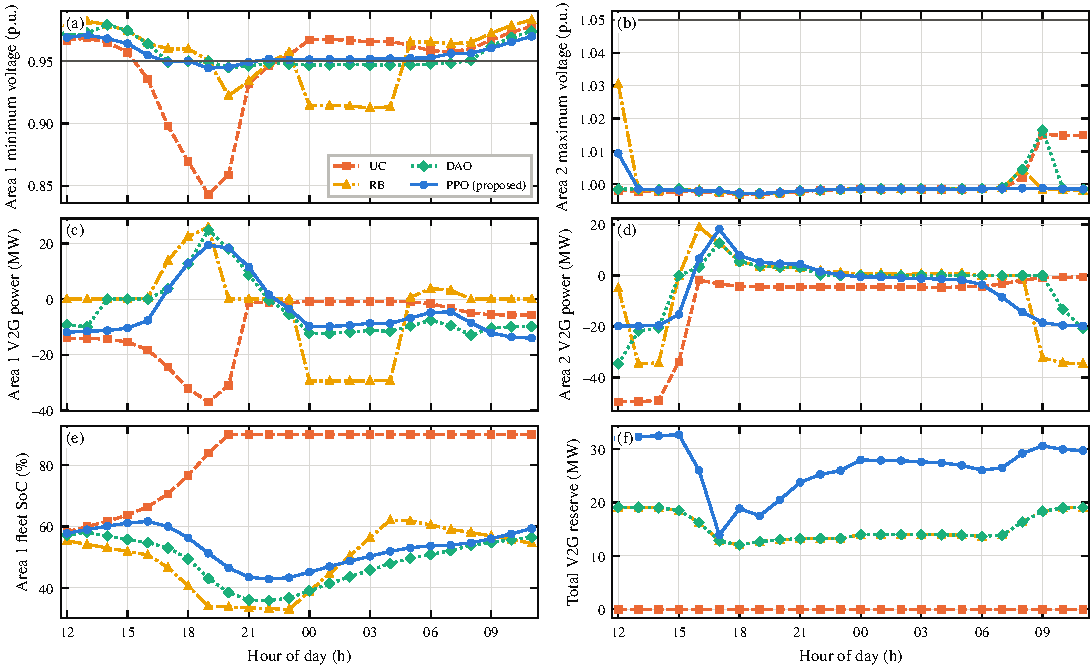
\includegraphics[width=\textwidth]{fig_day.pdf}
\caption{Representative test day (day 1, PPO seed 0). (a) Area~1
minimum bus voltage. (b) Area~2 maximum bus voltage. (c), (d) Area-level
V2G set-points (positive values denote discharge). (e) Area~1 fleet SoC.
(f) Total V2G frequency reserve.}
\label{fig:day}
\end{figure*}

\begin{figure*}[!t]
\centering
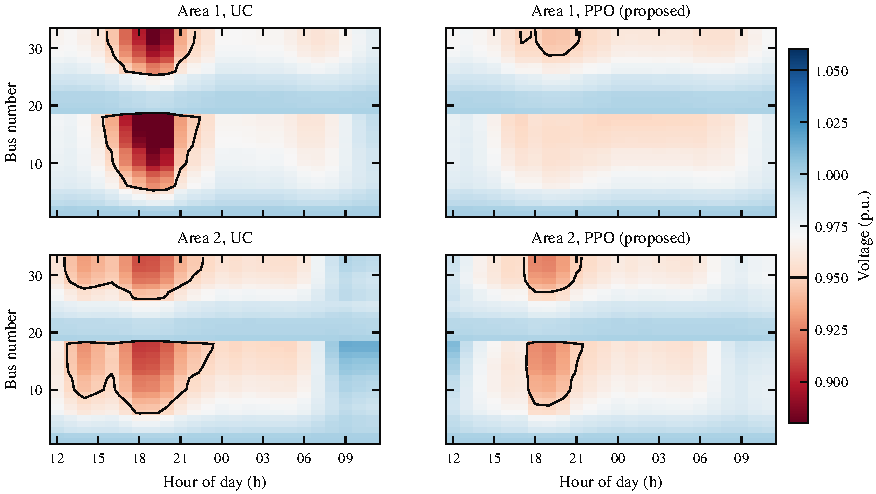
\includegraphics[width=0.9\textwidth]{fig_heatmap.pdf}
\caption{Bus voltages over the representative test day under UC and
PPO. Black contours mark 0.95 and 1.05~p.u.}
\label{fig:heatmap}
\end{figure*}

\subsection{Frequency Response Within an Hour}
\label{sec:freqres}

Fig.~\ref{fig:freq} shows the 60-s window at \FreqHour{} of the same
day. PV has reduced the inertia constant of Area~2 to \HrHtwo~s, and a
load step occurs in Area~1 at $t=2$~s; Area~2 sees the disturbance
through the tie line. Without reserve (UC), the Area~2 nadir
reaches \HrUCNadirTwo~mHz and the inter-area oscillation is lightly
damped. PPO holds \HrPPORes~MW of reserve at this hour, most of it in
Area~2 where the workplace fleet is connected, against \HrRBRes~MW for
RB. The Area~2 nadir is reduced to \HrPPONadirTwo~mHz (\HrRBNadirTwo~mHz with RB) and the oscillation
decays faster. The Area~1 nadir changes much less (\HrUCNadirOne, \HrRBNadirOne, and \HrPPONadirOne~mHz for UC,
RB, and PPO), because only about a quarter of the residential fleet is
plugged in at midday and PPO assigns it a small reserve share. The worst nadir over
the two areas in this hour is therefore \HrPPONadir~mHz for PPO and
\HrRBNadir~mHz for RB. This example shows that the benefit of reserve
depends on where the disturbance occurs relative to where the reserve
is held, which is why the test-set gains in Table~\ref{tab:test} are
averages over random disturbance locations.

\begin{figure*}[!t]
\centering
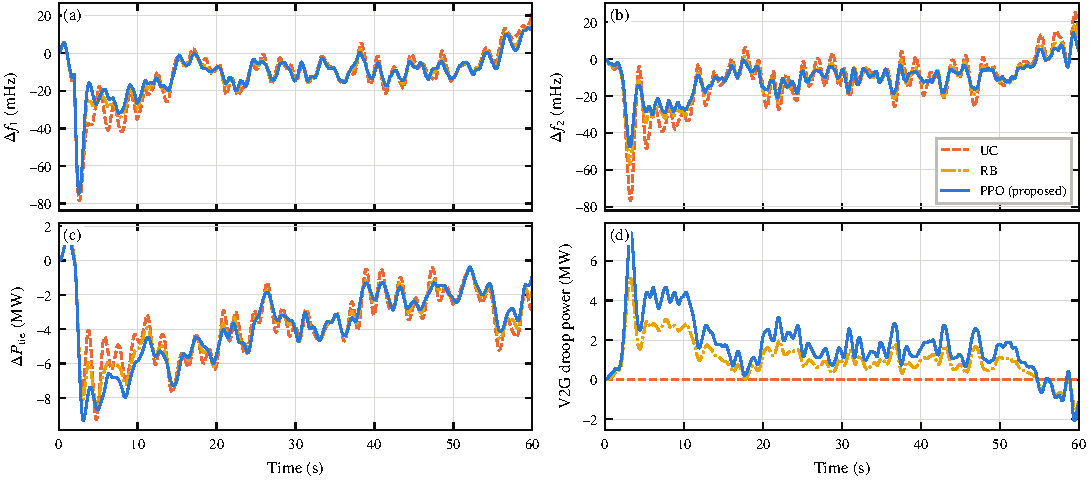
\includegraphics[width=\textwidth]{fig_freq.pdf}
\caption{Frequency response at \FreqHour{} of the representative day.
(a), (b) Area frequency deviations. (c) Tie-line power deviation.
(d) Total V2G droop power.}
\label{fig:freq}
\end{figure*}

\subsection{Learned Allocation Between Voltage Support and Reserve}
\label{sec:alloc}

Fig.~\ref{fig:policy} averages the PPO decisions over all test days and
seeds. The reserve share follows fleet availability more than inertia. In
Area~2, the policy holds $\rho\approx\RhoMidTwo$ between 10:00 and
14:00, when the workplace fleet is connected and PV has lowered the
inertia, and releases the reserve to zero in the evening, when the
few remaining vehicles are discharged to support the feeder voltage.
In Area~1, the reserve share is close to its upper limit at night
($\rho\approx\RhoNightOne$), when inertia is high but the residential
fleet is plugged in and otherwise idle, drops to \RhoMidOne{} at midday, when most
residential vehicles are away and the remaining ones charge, and settles
near \RhoEveOne{} during the evening peak, when part of the converter
capacity is used for discharge. The set-points show charging from
midday PV in both areas, discharge in the evening peak, and moderate
overnight charging in Area~1. None of these rules was specified in the
reward; they emerge from the trade-off encoded in \eqref{eq:cost}.

\begin{figure}[!t]
\centering
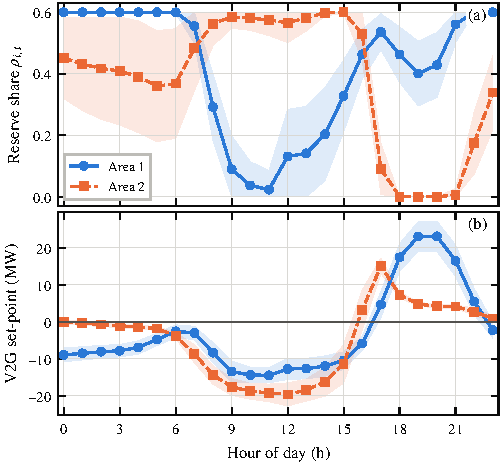
\includegraphics[width=\columnwidth]{fig_policy.pdf}
\caption{PPO decisions averaged over the test days and \NSeed{} seeds
(mean and $\pm1$ standard deviation). (a) Reserve share. (b) Area-level
V2G set-point.}
\label{fig:policy}
\end{figure}

\begin{figure*}[!t]
\centering
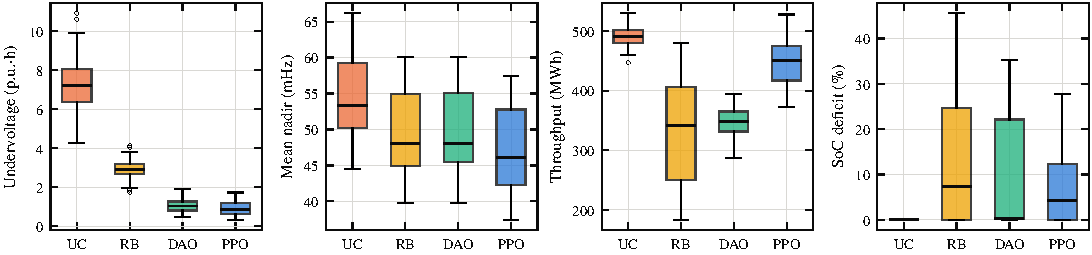
\includegraphics[width=\textwidth]{fig_box.pdf}
\caption{Distribution of daily metrics over the test days (PPO pooled
over \NSeed{} seeds).}
\label{fig:box}
\end{figure*}

Fig.~\ref{fig:box} shows the distributions behind the averages. The
undervoltage distribution of PPO lies below those of RB and DAO, and
its throughput is higher. Its mean SoC deficit is lower than that of RB
and DAO, but the median is not: DAO ends \TDAOSocDefZeroPct\% of the days with no
deficit (median \TDAOSocDefMedian\%), whereas PPO tends to leave a small deficit on many days (median \TPPOSocDefMedian\%). The nadir distributions of
all controllers overlap, because the day-to-day variation of the
disturbance size is larger than the effect of the reserve; compared
day by day, however, the PPO mean nadir is lower than that of DAO on
\TNadirWinsDAO{} of the 30 test days, than that of RB on \TNadirWinsRB,
and than that of UC on \TNadirWinsUC{} (paired Wilcoxon test against
DAO, $p=\TNadirPDAO$).

\subsection{Out-of-Distribution Stress Days}
\label{sec:stress}

Table~\ref{tab:stress} reports the 20 stress days, which combine 10\% to
20\% heavier load, 30\% to 45\% lower fleet participation, and larger
disturbances, all beyond the training ranges, with clear-sky PV. All controllers deteriorate. PPO remains the
lowest-cost controller, \SRedCostDAO\% below DAO and \SRedCostRB\% below
RB, and its daily cost is the lowest on all 20 days ($p=\SPDAO$ against
each benchmark). Its undervoltage is \SRedUvPuHDAO\% below DAO. The
policy does, however, show several signs of operating outside its
training range. It records more violation hours than RB
(\SPPOViolHours{} against \SRBViolHours), because it spreads the
limited fleet energy over more hours with shallow violations, its
terminal SoC deficit rises to \SPPOSocDefPct\%, and its maximum voltage
reaches \SPPOVmaxDay~p.u. Training on a wider scenario distribution, or
adding a hard terminal-energy constraint, would be needed before
deployment under such conditions.

\begin{table*}[!t]
\caption{Results on the 20 out-of-distribution stress days (mean $\pm$ standard deviation across days). PPO values are pooled over 5 seeds; the value in parentheses is the standard deviation of the per-seed means.}
\label{tab:stress}
\centering
\footnotesize
\begin{tabular}{lcccc}
\toprule
\textbf{Metric} & \textbf{UC} & \textbf{RB} & \textbf{DAO} & \textbf{PPO (proposed)}\\
\midrule
Daily cost $\sum_t c_t$ & 671.4 $\pm$ 24.3 & 369.4 $\pm$ 17.6 & 308.3 $\pm$ 19.6 & 283.8 $\pm$ 16.2 (3.1) \\
Voltage-violation hours (h) & 24.3 $\pm$ 2.3 & 14.2 $\pm$ 1.3 & 18.6 $\pm$ 4.5 & 18.5 $\pm$ 3.0 (1.0) \\
Undervoltage (p.u.$\cdot$h) & 10.25 $\pm$ 0.50 & 4.15 $\pm$ 0.36 & 2.88 $\pm$ 0.29 & 2.66 $\pm$ 0.27 (0.13) \\
Overvoltage (p.u.$\cdot$h) & 0.070 $\pm$ 0.024 & 0.000 $\pm$ 0.001 & 0.000 $\pm$ 0.001 & 0.006 $\pm$ 0.009 (0.003) \\
Minimum voltage (p.u.) & 0.835 $\pm$ 0.006 & 0.898 $\pm$ 0.003 & 0.903 $\pm$ 0.004 & 0.905 $\pm$ 0.004 (0.000) \\
Maximum voltage (p.u.) & 1.070 $\pm$ 0.004 & 1.043 $\pm$ 0.005 & 1.048 $\pm$ 0.002 & 1.052 $\pm$ 0.005 (0.002) \\
Mean hourly nadir (mHz) & 82.6 $\pm$ 6.4 & 76.8 $\pm$ 6.2 & 77.6 $\pm$ 6.3 & 75.0 $\pm$ 6.1 (0.4) \\
Worst nadir (mHz) & 121.3 $\pm$ 11.5 & 108.6 $\pm$ 9.9 & 108.6 $\pm$ 10.0 & 105.8 $\pm$ 9.3 (0.5) \\
Maximum RoCoF (Hz/s) & 0.240 $\pm$ 0.021 & 0.215 $\pm$ 0.018 & 0.215 $\pm$ 0.018 & 0.205 $\pm$ 0.019 (0.002) \\
Terminal SoC deficit (\%) & 0.00 $\pm$ 0.00 & 26.16 $\pm$ 3.65 & 24.30 $\pm$ 8.70 & 18.02 $\pm$ 4.07 (2.94) \\
Projection events per day & 16.4 $\pm$ 1.0 & 0.0 $\pm$ 0.0 & 2.8 $\pm$ 3.0 & 0.0 $\pm$ 0.0 (0.0) \\
Unmet mobility energy (MWh) & 0.00 $\pm$ 0.00 & 0.00 $\pm$ 0.00 & 2.43 $\pm$ 2.76 & 0.00 $\pm$ 0.00 (0.00) \\
\bottomrule
\end{tabular}
\end{table*}


\subsection{Reward Ablation and Weight Sensitivity}
\label{sec:ablation}

Tables~\ref{tab:ablation} and \ref{tab:sensitivity} report policies
trained with one reward term removed, or with the voltage or frequency
weight halved and doubled, and evaluated with the nominal cost
\eqref{eq:cost}. To limit computation each variant was trained for
200\,000 steps, with three seeds for the ablation and two for the
sensitivity study, and a reference policy with the nominal reward was
trained under the same budget in the same environment.
The comparison is made against this reference, not against the
400\,000-step policies of Table~\ref{tab:test}. The same seed means
the same initial network weights and the same scenario stream, so the
seed-paired difference between a variant and the reference isolates the
effect of the reward change.

\emph{Frequency terms.} Removing them has a clear and consistent
effect. All three seeds give up most of the reserve
(\AblNoFReserveMeanMw~MW instead of \AblRefReserveMeanMw~MW), raise the
mean nadir from \AblRefNadirMeanHz{} to \AblNoFNadirMeanHz~mHz, and
increase the nominal cost in every seed pair (differences
\AblNoFPairDiffs; mean \AblNoFPairMean). Halving $w_f$ moves the policy
in the same direction (reserve \AblWfLowReserveMeanMw~MW, paired cost
differences \AblWfLowPairDiffs), and doubling it raises the reserve to
\AblWfHighReserveMeanMw~MW at the price of more undervoltage
(\AblWfHighUvPuH~p.u.$\cdot$h against \AblRefUvPuH). The reserve
allocation of Fig.~\ref{fig:policy} is therefore controlled by the
frequency weight, and the nominal $w_f=4$ sits between the two extremes.

\emph{Voltage weight.} Doubling $w_V$ reduces undervoltage to
\AblWvHighUvPuH~p.u.$\cdot$h but cuts the reserve by
\AblWvHighReserveRedPct\% (\AblWvHighReserveMeanMw~MW) and raises the terminal SoC deficit to
\AblWvHighSocDefPct\%, because the policy discharges more in the evening
and recharges less. Halving $w_V$ does the opposite. The two weights
thus trade voltage support against reserve and end-of-day energy in the
expected directions.

\emph{Why some variants show a lower total cost than the reference.}
Removing the overvoltage or throughput term, halving $w_V$, or
doubling $w_f$ yields a lower mean nominal cost than the reference
(Tables~\ref{tab:ablation} and \ref{tab:sensitivity}),
which at first sight suggests that these terms are harmful. The cost
decomposition shows otherwise. The voltage, frequency, and throughput
components of the reference and of these variants differ by only a few
units (voltage \AblRefCostV{} against \AblNoOVCostV{} and
\AblNoDegCostV; frequency \AblRefCostF{} against \AblNoOVCostF{} and
\AblNoDegCostF). Almost the entire difference comes from the terminal
SoC term, which is \AblRefCostTerm{} for the reference,
\AblNoOVCostTerm{} without the overvoltage term, \AblNoDegCostTerm{}
without the throughput term, \AblWvLowCostTerm{} with $w_V=25$, and
\AblWfHighCostTerm{} with $w_f=8$. This
term is paid once per episode and is the slowest part of the reward to
learn: at 200\,000 steps the three reference seeds leave terminal
deficits of \AblRefSeedSocDefs{} percentage points (seed costs
\AblRefSeedCosts), whereas the 400\,000-step policies of
Table~\ref{tab:test} reach \TPPOSocDefPct\%. The apparent advantage of the variants is therefore a
training-budget effect on a term unrelated to the removed one, and it is
not statistically distinguishable from the reference (Welch tests on
seed means, $p=\AblNoOVPval$ and $p=\AblNoDegPval$; paired differences
\AblNoOVPairDiffs{} and \AblNoDegPairDiffs). Consistent with this, the
200\,000-step runs with large terminal deficits have not met the
convergence criterion of Section~\ref{sec:ppo} (validation cost still
changing by up to \AblNoOVConvMax\% over the final 50\,000 steps). The
overvoltage term has little effect on the test days because
overvoltage is rare for every policy, and the throughput term with
$w_{\mathrm{deg}}=0.05$ is a minor part of the cost. We keep both terms
because they encode constraints that matter on days the test set does
not represent, but the evidence here does not show that they improve
performance.

\begin{table*}[!t]
\caption{Reward ablation on the test days (mean $\pm$ standard deviation across seeds). Every policy is trained for 200\,000 steps in the corrected environment with the modified reward and evaluated with the full cost \eqref{eq:cost}.}
\label{tab:ablation}
\centering
\footnotesize
\setlength{\tabcolsep}{4pt}
\begin{tabular}{lccccccc}
\toprule
\textbf{Reward variant (seeds)} & \textbf{Cost} & \textbf{UV (p.u.$\cdot$h)} & \textbf{OV (p.u.$\cdot$h)} & \textbf{Nadir (mHz)} & \textbf{Reserve (MW)} & \textbf{Thr. (MWh)} & \textbf{SoC def. (\%)}\\
\midrule
Full reward (reference) (3) & 147.3 $\pm$ 10.7 & 0.92 $\pm$ 0.03 & 0.003 $\pm$ 0.002 & 47.8 $\pm$ 0.4 & 22.9 $\pm$ 2.6 & 437 $\pm$ 25 & 15.62 $\pm$ 10.68 \\
$w_{\mathrm{ov}}=0$ (no overvoltage term) (3) & 144.4 $\pm$ 5.4 & 0.92 $\pm$ 0.02 & 0.004 $\pm$ 0.001 & 47.5 $\pm$ 0.2 & 24.4 $\pm$ 0.5 & 431 $\pm$ 32 & 13.75 $\pm$ 7.06 \\
$w_f=w_{\mathrm{tie}}=0$ (no frequency terms) (3) & 169.0 $\pm$ 0.9 & 0.86 $\pm$ 0.01 & 0.001 $\pm$ 0.000 & 51.0 $\pm$ 0.4 & 10.1 $\pm$ 1.3 & 512 $\pm$ 29 & 28.68 $\pm$ 0.36 \\
$w_{\mathrm{deg}}=0$ (no throughput term) (3) & 145.6 $\pm$ 10.3 & 0.92 $\pm$ 0.03 & 0.002 $\pm$ 0.001 & 47.8 $\pm$ 0.3 & 23.1 $\pm$ 1.9 & 452 $\pm$ 23 & 13.88 $\pm$ 10.75 \\
\bottomrule
\end{tabular}
\end{table*}

\begin{table*}[!t]
\caption{Reward-weight sensitivity on the test days (mean $\pm$ standard deviation across seeds; 200\,000 steps; evaluation with the nominal weights of Table~\ref{tab:params}).}
\label{tab:sensitivity}
\centering
\footnotesize
\setlength{\tabcolsep}{4pt}
\begin{tabular}{lccccccc}
\toprule
\textbf{Reward variant (seeds)} & \textbf{Cost} & \textbf{UV (p.u.$\cdot$h)} & \textbf{OV (p.u.$\cdot$h)} & \textbf{Nadir (mHz)} & \textbf{Reserve (MW)} & \textbf{Thr. (MWh)} & \textbf{SoC def. (\%)}\\
\midrule
Full reward (reference) (3) & 147.3 $\pm$ 10.7 & 0.92 $\pm$ 0.03 & 0.003 $\pm$ 0.002 & 47.8 $\pm$ 0.4 & 22.9 $\pm$ 2.6 & 437 $\pm$ 25 & 15.62 $\pm$ 10.68 \\
$w_V=25$ (half) (2) & 140.1 $\pm$ 0.4 & 1.09 $\pm$ 0.03 & 0.008 $\pm$ 0.003 & 47.0 $\pm$ 0.1 & 26.4 $\pm$ 0.4 & 428 $\pm$ 3 & 2.17 $\pm$ 0.78 \\
$w_V=100$ (double) (2) & 167.5 $\pm$ 0.4 & 0.85 $\pm$ 0.01 & 0.003 $\pm$ 0.002 & 49.9 $\pm$ 0.1 & 13.9 $\pm$ 0.3 & 442 $\pm$ 19 & 30.85 $\pm$ 0.28 \\
$w_f=2$ (half) (2) & 161.9 $\pm$ 5.8 & 0.87 $\pm$ 0.00 & 0.001 $\pm$ 0.001 & 49.3 $\pm$ 0.8 & 16.5 $\pm$ 3.4 & 458 $\pm$ 30 & 27.38 $\pm$ 2.56 \\
$w_f=8$ (double) (2) & 140.5 $\pm$ 0.4 & 1.00 $\pm$ 0.01 & 0.007 $\pm$ 0.001 & 46.9 $\pm$ 0.4 & 26.6 $\pm$ 1.3 & 415 $\pm$ 21 & 7.84 $\pm$ 0.90 \\
\bottomrule
\end{tabular}
\end{table*}


\subsection{Limitations}
\label{sec:limits}

Several simplifications bound the conclusions. Each area's
distribution system is represented by identical copies of one feeder,
so feeder diversity and the coupling between distribution voltages and
transmission-level frequency are not captured. The fleet is modeled as
one aggregated battery per feeder; individual departure constraints,
charger heterogeneity, and battery aging physics are not modeled, and
the throughput term is only a proxy for degradation. Reactive-power
capability of the chargers, which is effective for voltage control
\cite{HuEtAl2022}, is not used. The load, PV, and availability profiles
are synthetic, and the LFC model is linearized with representative
parameters rather than identified from a specific system. Finally, the
agent receives hour-ahead forecasts without error; forecast
uncertainty and communication delays at the aggregator level are left
for future work.

% ============================================================
\section{Conclusion}
\label{sec:conclusions}
% ============================================================

This paper formulated the coordination of V2G voltage support and
frequency reserve as a two-time-scale control problem and solved it
with PPO. The hourly decision of each area aggregator consists of a
fleet set-point and a reserve share. The set-point is evaluated by AC
power flow on IEEE 33-bus feeders and an energy-consistent fleet model,
and the reserve determines the gain and saturation of a V2G droop loop
in a dynamic two-area LFC model with inertia, governors, a tie line,
and AGC. All quantities are expressed in physical units, and the
models were verified against pandapower and closed-form results.

Across \NSeed{} training seeds and 30 held-out days, the learned policy
reduced the daily cost by \TRedCostDAO\% relative to a perfect-foresight
day-ahead optimization with fixed reserve, by \TRedCostRB\% relative to
a rule-based volt-watt and droop controller, and by \TRedCostUC\%
relative to uncontrolled charging. Undervoltage fell by
\TRedUvPuHDAO\% relative to the day-ahead optimization, the mean
frequency nadir by \TRedNadirMeanHzDAO\%, and the terminal SoC deficit
from \TDAOSocDefPct\% to \TPPOSocDefPct\%. The policy learned to hold
reserve mainly where and when vehicles are plugged in, including the
low-inertia midday hours in the workplace area, and to release it when
converter capacity is needed for voltage support. On
out-of-distribution stress days the policy kept the lowest cost but
showed larger SoC deficits and more frequent shallow violations,
which marks the limits of the training distribution.

Future work will add charger reactive power, forecast uncertainty,
heterogeneous feeders, electricity-cost terms in the objective, and
constrained RL formulations that enforce terminal energy requirements
as hard constraints.

\section*{Data and Code Availability}
The simulation environment, training and evaluation scripts, trained
policies, and the data behind every table and figure are available at
\url{https://github.com/kenoto99/v2g-ppo-two-area} (release v3.0.1;
archived on Zenodo, DOI: \url{https://doi.org/10.5281/zenodo.23851585}).

\section*{Acknowledgment}
The authors used an AI assistant (Claude, Anthropic) to help implement
and debug the simulation code and to edit the language of the
manuscript. All models, parameters, results, and interpretations were
checked by the authors, who take full responsibility for the content.


\begin{thebibliography}{99}

\bibitem{Kempton2005}
W. Kempton and J. Tomic,
``Vehicle-to-grid power fundamentals: Calculating capacity and net revenue,''
\emph{J. Power Sources}, vol. 144, pp. 268--279, 2005,
doi: 10.1016/j.jpowsour.2004.12.025.

\bibitem{BaranWu1989}
M. E. Baran and F. F. Wu,
``Network reconfiguration in distribution systems for loss reduction
and load balancing,''
\emph{IEEE Trans. Power Del.}, vol. 4, no. 2, pp. 1401--1407, 1989,
doi: 10.1109/61.25627.

\bibitem{YenchamchalitEtAl2018PSO}
K. Yenchamchalit, Y. Kongjeen, K. Bhumkittipich,
and N. Mithulananthan,
``Optimal sizing and location of the charging station for plug-in
electric vehicles using the particle swarm optimization technique,''
in \emph{Proc. 2018 Int. Electr. Eng. Congr. (iEECON)},
Krabi, Thailand, Mar. 7--9, 2018, pp. 524--527,
doi: 10.1109/IEECON.2018.8712336.

\bibitem{YenchamchalitEtAl2021LFO}
K. Yenchamchalit, Y. Kongjeen, K. Bhumkittipich, A. Stativa,
and N. Mithulananthan,
``Control of low-frequency oscillation on electrical power system
under large EV-charging station installation using PSO technique
for turning PSS parameters,''
\emph{Int. Rev. Electr. Eng. (IREE)},
vol. 16, no. 5, pp. 401--408, 2021,
doi: 10.15866/iree.v16i5.20753.

\bibitem{Yenchamchalit2021}
K. Yenchamchalit, Y. Kongjeen, P. Prabpal, and K. Bhumkittipich,
``Optimal placement of distributed photovoltaic systems and electric
vehicle charging stations using metaheuristic optimization techniques,''
\emph{Symmetry}, vol. 13, Art. no. 2378, 2021,
doi: 10.3390/sym13122378.

\bibitem{Kongjeen2019}
Y. Kongjeen, K. Bhumkittipich, and N. Mithulananthan,
``Optimal DG sizing and location in modern power grids using PEVs
load demand probability,''
\emph{ECTI Trans. Electr. Eng. Electron. Commun.},
vol. 17, no. 1, pp. 51--59, 2019,
doi: 10.37936/ecti-eec.2019171.215410.

\bibitem{Nuamkoksung2025}
P. Nuamkoksung, W. Sanga-ngam, K. Suthamno, T. Klayklueng,
S. Marsong, S. Sonasang, K. Bhumkittipich, D. N. Vo, K. Buayai,
K. Kerdchuen, and Y. Kongjeen,
``Integrated control of DER placement and network reconfiguration in
EV-charging distribution systems using multi-optimization techniques,''
\emph{Engineering Access}, vol. 11, pp. 301--318, 2025,
doi: 10.14456/mijet.2025.31.

\bibitem{Sortomme2011}
E. Sortomme and M. A. El-Sharkawi,
``Optimal charging strategies for unidirectional vehicle-to-grid,''
\emph{IEEE Trans. Smart Grid}, vol. 2, no. 1, pp. 131--138,
Mar. 2011,
doi: 10.1109/TSG.2010.2090910.

\bibitem{Lam2016}
A. Y. S. Lam, K.-C. Leung, and V. O. K. Li,
``Capacity estimation for vehicle-to-grid frequency regulation services
with smart charging mechanism,''
\emph{IEEE Trans. Smart Grid}, vol. 7, no. 1, pp. 156--166,
Jan. 2016,
doi: 10.1109/TSG.2015.2436901.

\bibitem{AmamraMarco2019}
S.-A. Amamra and J. Marco,
``Vehicle-to-grid aggregator to support power grid and reduce electric
vehicle charging cost,''
\emph{IEEE Access}, vol. 7, pp. 178528--178538, 2019,
doi: 10.1109/ACCESS.2019.2958664.

\bibitem{HuEtAl2022}
J. Hu \emph{et al.},
``A distributed MPC to exploit reactive power V2G for real-time voltage
regulation in distribution networks,''
\emph{IEEE Trans. Smart Grid}, vol. 13, no. 1, pp. 576--588,
Jan. 2022,
doi: 10.1109/TSG.2021.3109453.

\bibitem{AnEtAl2024}
H. An \emph{et al.},
``A robust V2G voltage control scheme for distribution networks against
cyber attacks and customer interruptions,''
\emph{IEEE Trans. Smart Grid}, vol. 15, no. 4, pp. 3966--3978,
Jul. 2024,
doi: 10.1109/TSG.2024.3365069.

\bibitem{YuanEtAl2026}
Z. Yuan, J. Feng, Y. Shi, and J. Cort{\'e}s,
``Stability constrained voltage control in distribution grids with
arbitrary communication infrastructure,''
\emph{IEEE Trans. Smart Grid}, vol. 17, no. 1, pp. 351--362,
Jan. 2026,
doi: 10.1109/TSG.2025.3610124.

\bibitem{YanXu2020}
Z. Yan and Y. Xu,
``A multi-agent deep reinforcement learning method for cooperative
load frequency control of a multi-area power system,''
\emph{IEEE Trans. Power Syst.}, vol. 35, pp. 4599--4608, 2020,
doi: 10.1109/TPWRS.2020.2999890.

\bibitem{Abouheaf2019}
M. Abouheaf, W. Gueaieb, and A. M. Sharaf,
``Load frequency regulation for multi-area power system using integral
reinforcement learning,''
\emph{IET Gener. Transm. Distrib.},
vol. 13, no. 19, pp. 4311--4323, Oct. 2019,
doi: 10.1049/iet-gtd.2019.0218.

\bibitem{Alfaverh2023}
F. Alfaverh, M. Denai, and Y. Sun,
``Optimal vehicle-to-grid control for supplementary frequency regulation
using deep reinforcement learning,''
\emph{Electr. Power Syst. Res.},
vol. 214, Art. no. 108949, 2023,
doi: 10.1016/j.epsr.2022.108949.

\bibitem{MaHuSong2024}
Y. Ma, Z. Hu, and Y. Song,
``A reinforcement learning based coordinated but differentiated load
frequency control method with heterogeneous frequency regulation resources,''
\emph{IEEE Trans. Power Syst.}, vol. 39, pp. 2239--2250, 2024,
doi: 10.1109/TPWRS.2023.3262543.

\bibitem{ZhaoLiuHill2025}
Y. Zhao, T. Liu, and D. J. Hill,
``Distributed attention-enabled multi-agent reinforcement learning based
frequency regulation of power systems,''
\emph{IEEE Trans. Power Syst.}, vol. 40, pp. 2427--2437, 2025,
doi: 10.1109/TPWRS.2024.3469132.

\bibitem{Wu2024Symmetry}
M. Wu, D. Ma, K. Xiong, and L. Yuan,
``Deep reinforcement learning for load frequency control in isolated
microgrids: A knowledge aggregation approach with emphasis on power
symmetry and balance,''
\emph{Symmetry}, vol. 16, Art. no. 322, 2024,
doi: 10.3390/sym16030322.

\bibitem{Liang2026Symmetry}
C. Liang,
``Distributed V2G grid frequency regulation considering EV owner
participation via cooperative integral reinforcement learning,''
\emph{Symmetry}, vol. 18, Art. no. 824, 2026,
doi: 10.3390/sym18050824.

\bibitem{Xiong2026Symmetry}
X. Xiong, S. Li, K. Xia, H. Zheng, Z. Huang, T. Zhu, Z. Wang,
and Q. Kang,
``Spatially heterogeneous resilient V2G-enabled grid frequency control
via an adversarially trained structural switching framework,''
\emph{Symmetry}, vol. 18, Art. no. 843, 2026,
doi: 10.3390/sym18050843.

\bibitem{AbazariEtAl2025}
A. Abazari, M. Ghafouri, D. Jafarigiv, R. Atallah, and C. Assi,
``Data-driven framework for mitigating EV-based load-altering attacks
on LFC model of microgrid,''
\emph{IEEE Trans. Consum. Electron.}, vol. 71, no. 2,
pp. 6093--6108, May 2025,
doi: 10.1109/TCE.2025.3563392.

\bibitem{Schulman2017}
J. Schulman, F. Wolski, P. Dhariwal, A. Radford, and O. Klimov,
``Proximal policy optimization algorithms,''
\emph{arXiv preprint arXiv:1707.06347}, 2017.

\bibitem{Izadkhast2015}
S. Izadkhast, P. Garcia-Gonzalez, and P. Fr\'{\i}as,
``An aggregate model of plug-in electric vehicles for primary frequency control,''
\emph{IEEE Trans. Power Syst.}, vol. 30, no. 3, pp. 1475--1482, May 2015,
doi: 10.1109/TPWRS.2014.2337373.

\bibitem{Izadkhast2016}
S. Izadkhast, P. Garcia-Gonzalez, P. Fr\'{\i}as, L. Ram\'{\i}rez-Elizondo, and P. Bauer,
``An aggregate model of plug-in electric vehicles including distribution network
characteristics for primary frequency control,''
\emph{IEEE Trans. Power Syst.}, vol. 31, no. 4, pp. 2987--2998, Jul. 2016,
doi: 10.1109/TPWRS.2015.2471091.

\bibitem{Tielens2016}
P. Tielens and D. Van Hertem,
``The relevance of inertia in power systems,''
\emph{Renew. Sustain. Energy Rev.}, vol. 55, pp. 999--1009, 2016,
doi: 10.1016/j.rser.2015.11.016.

\bibitem{Cao2022}
D. Cao, J. Zhao, W. Hu, N. Yu, F. Ding, Q. Huang, and Z. Chen,
``Deep reinforcement learning enabled physical-model-free two-timescale voltage
control method for active distribution systems,''
\emph{IEEE Trans. Smart Grid}, vol. 13, no. 1, pp. 149--165, Jan. 2022,
doi: 10.1109/TSG.2021.3113085.

\bibitem{Thurner2018}
L. Thurner, A. Scheidler, F. Sch\"{a}fer, J.-H. Menke, J. Dollichon, F. Meier,
S. Meinecke, and M. Braun,
``pandapower: An open-source Python tool for convenient modeling, analysis, and
optimization of electric power systems,''
\emph{IEEE Trans. Power Syst.}, vol. 33, no. 6, pp. 6510--6521, Nov. 2018,
doi: 10.1109/TPWRS.2018.2829021.

\bibitem{Teng2003}
J.-H. Teng,
``A direct approach for distribution system load flow solutions,''
\emph{IEEE Trans. Power Del.}, vol. 18, no. 3, pp. 882--887, Jul. 2003,
doi: 10.1109/TPWRD.2003.813818.

\bibitem{Kundur1994}
P. Kundur, \emph{Power System Stability and Control}.
New York, NY, USA: McGraw-Hill, 1994.

\bibitem{Bevrani2014}
H. Bevrani, \emph{Robust Power System Frequency Control}, 2nd ed.
Cham, Switzerland: Springer, 2014,
doi: 10.1007/978-3-319-07278-4.

\bibitem{Raffin2021}
A. Raffin, A. Hill, A. Gleave, A. Kanervisto, M. Ernestus, and N. Dormann,
``Stable-Baselines3: Reliable reinforcement learning implementations,''
\emph{J. Mach. Learn. Res.}, vol. 22, no. 268, pp. 1--8, 2021.

\bibitem{Raffin2022}
A. Raffin, J. Kober, and F. Stulp,
``Smooth exploration for robotic reinforcement learning,''
in \emph{Proc. 5th Conf. Robot Learn. (CoRL)}, PMLR vol. 164, 2022, pp. 1634--1644.

\bibitem{Schulman2016}
J. Schulman, P. Moritz, S. Levine, M. Jordan, and P. Abbeel,
``High-dimensional continuous control using generalized advantage estimation,''
in \emph{Proc. Int. Conf. Learn. Represent. (ICLR)}, 2016,
arXiv:1506.02438.

\bibitem{Henderson2018}
P. Henderson, R. Islam, P. Bachman, J. Pineau, D. Precup, and D. Meger,
``Deep reinforcement learning that matters,''
in \emph{Proc. AAAI Conf. Artif. Intell.}, vol. 32, no. 1, 2018,
pp. 3207--3214, doi: 10.1609/aaai.v32i1.11694.

\bibitem{Jardini2000}
J. A. Jardini, C. M. V. Tahan, M. R. Gouvea, S. U. Ahn, and F. M. Figueiredo,
``Daily load profiles for residential, commercial and industrial low voltage
consumers,''
\emph{IEEE Trans. Power Del.}, vol. 15, no. 1, pp. 375--380, Jan. 2000,
doi: 10.1109/61.847276.

\bibitem{Schey2012}
S. Schey, D. Scoffield, and J. Smart,
``A first look at the impact of electric vehicle charging on the electric grid
in The EV Project,''
\emph{World Electr. Veh. J.}, vol. 5, no. 3, pp. 667--678, 2012,
doi: 10.3390/wevj5030667.

\bibitem{INL2014}
Idaho National Laboratory,
``Workplace charging frequency of Nissan Leafs and Chevrolet Volts in The EV
Project at six work sites,''
Idaho Falls, ID, USA, Tech. Rep., Nov. 2014. [Online]. Available:
https://avt.inl.gov/sites/default/files/pdf/EVProj/ChargingAtSixWorkSites.pdf

\bibitem{Donati2015}
A. V. Donati, P. Dilara, C. Thiel, A. Spadaro, D. Gkatzoflias, and Y. Drossinos,
\emph{Individual Mobility: From Conventional to Electric Cars},
Publications Office of the European Union, Luxembourg, Rep. EUR 27468 EN,
2015, doi: 10.2790/405373.

\bibitem{KoSung2018}
K. S. Ko and D. K. Sung,
``The effect of EV aggregators with time-varying delays on the stability of a
load frequency control system,''
\emph{IEEE Trans. Power Syst.}, vol. 33, no. 1, pp. 669--680, Jan. 2018,
doi: 10.1109/TPWRS.2017.2690915.

\bibitem{Ziras2017}
C. Ziras, J. Hu, S. You, and H. W. Bindner,
``Modelling the aggregated dynamic response of electric vehicles,''
in \emph{Proc. IEEE PES Innov. Smart Grid Technol. Conf. Eur. (ISGT-Europe)},
Torino, Italy, Sep. 2017, pp. 1--6, doi: 10.1109/ISGTEurope.2017.8260222.

\bibitem{Bishop2013}
J. D. K. Bishop, C. J. Axon, D. Bonilla, M. Tran, D. Banister, and M. D. McCulloch,
``Evaluating the impact of V2G services on the degradation of batteries in PHEV
and EV,''
\emph{Appl. Energy}, vol. 111, pp. 206--218, Nov. 2013,
doi: 10.1016/j.apenergy.2013.04.094.

\end{thebibliography}


\begin{IEEEbiography}[{\authorphoto{A1.jpg}}]{SONTAYA MANMAI}
(Student Member, IEEE) received the B.IET. degree in Industrial
Electrical Technology from King Mongkut's Institute of Technology
North Bangkok, Thailand, in 2000, and the M.EE. degree in electrical
power from Rajamangala University of Technology Thanyaburi (RMUTT),
Pathum Thani, Thailand, in 2012.

He is currently with the Department of Electrical Engineering,
Faculty of Engineering, Rajamangala University of Technology
Thanyaburi, Pathum Thani, Thailand. His research interests include
power and energy systems, renewable-energy integration, electric
vehicles, power-system stability assessment and prediction, and
smart and flexible power grids.
\end{IEEEbiography}


\begin{IEEEbiography}[{\authorphoto{A2.png}}]{PRAKASIT PRABPAL}
received the B.Eng. degree in Electrical Engineering from
Khon Kaen University (KKU), Khon Kaen, Thailand, in 2008,
the M.Eng. degree in Electrical and Computer Engineering from
Mahasarakham University (MSU), Maha Sarakham, Thailand, in 2011,
and the D.Eng. degree in Electrical Engineering from Rajamangala
University of Technology Thanyaburi (RMUTT), Pathum Thani,
Thailand, in 2021.

He is currently with the Department of Electrical Technology,
Udon Thani Technical College, Institute of Vocational Education
Northeastern Region 1, Udon Thani, Thailand. His research interests
include electrical power systems, power-system dynamics, energy
storage, electric vehicles, vehicle-to-grid applications, smart-grid
operation, and optimization techniques for modern power and energy
systems.
\end{IEEEbiography}


\begin{IEEEbiography}[{\authorphoto{A3.png}}]{YUTTANA KONGJEEN}
received the B.Eng. and M.Eng. degrees in Electrical Engineering
from Rajamangala University of Technology Isan (RMUTI),
Nakhon Ratchasima, Thailand, and the D.Eng. degree from
Rajamangala University of Technology Thanyaburi (RMUTT),
Pathum Thani, Thailand.

He is currently an Assistant Professor with the Department of
Electrical Engineering, Faculty of Engineering and Technology,
Rajamangala University of Technology Isan, Nakhon Ratchasima,
Thailand. He is also a member of the Intelligent Power System and
Energy Research (IPER) group. His research interests include
power-system optimization, electric vehicles, distribution systems,
energy storage, microgrids, energy management, power-system
stability, and renewable-energy integration.
\end{IEEEbiography}


\begin{IEEEbiography}[{\authorphoto{A4.jpg}}]{WASAN PHETPHIMOON}
received the M.Eng. and D.Eng. degrees in Electrical Engineering
from Rajamangala University of Technology Thanyaburi (RMUTT),
Pathum Thani, Thailand.

He is currently an Assistant Professor with the Department of
Electrical Engineering Technology, Faculty of Industrial Technology,
Kamphaeng Phet Rajabhat University, Kamphaeng Phet, Thailand.
His research interests include power electronics, high-frequency
power converters, renewable-energy conversion, photovoltaic systems,
battery-charging converters, bidirectional dc--dc converters,
electric vehicles, and energy-storage applications.
\end{IEEEbiography}


\begin{IEEEbiography}[{\authorphoto{A5.png}}]{KULSOMSUP YENCHAMCHALIT}
received the B.Ind.Tech. degree in Electrical Industrial Technology
from Thepsatri Rajabhat University, Thailand, in 2001, the M.Eng.
degree in Electrical Engineering from Mahanakorn University of
Technology, Thailand, in 2010, and the D.Eng. degree in Electrical
Engineering from Rajamangala University of Technology Thanyaburi,
Pathum Thani, Thailand, in 2022.

She is currently a Lecturer with the Department of Electrical
Industrial Technology, Faculty of Industrial Technology, Thepsatri
Rajabhat University, Lopburi, Thailand, where she also serves as
Deputy Dean for Administration. Her research interests include
electrical power systems, distributed energy resources, renewable-
energy integration, electric vehicles, and intelligent control
applications in modern power systems.
\end{IEEEbiography}


\begin{IEEEbiography}[{\authorphoto{A6.png}}]{SOMCHAT SONASANG}
(Member, IEEE) was born in Nongbua Lamphu, Thailand. He received
the B.Eng. degree in Electronics and Telecommunication Engineering
from Rajamangala University of Technology Isan (RMUTI),
Nakhon Ratchasima Campus, Thailand, in 2006, the M.Eng. degree
in Electrical Engineering from Khon Kaen University (KKU),
Khon Kaen, Thailand, in 2009, and the Ph.D. degree in Electrical
and Computer Engineering from Mahasarakham University (MSU),
Maha Sarakham, Thailand, in 2021.

He is currently an Associate Professor with the Faculty of
Industrial Technology, Nakhon Phanom University, Nakhon Phanom,
Thailand, and is affiliated with the Electrical Elements and
Wireless Devices Unit (EEWDU). His research interests include
microwave circuits and devices, electromagnetic material
characterization, nondestructive microwave sensing, antennas,
and applied electromagnetics. His recent research interests also
include renewable-energy systems, electric vehicles, vehicle-to-grid
integration, intelligent optimization, and computational methods
for modern power and energy systems.
\end{IEEEbiography}


\begin{IEEEbiography}[{\authorphoto{A7.jpg}}]{KRISCHONME BHUMKITTIPICH}
received the B.Eng. degree in Electrical Power Engineering
from Rajamangala University of Technology Thanyaburi (RMUTT),
Pathum Thani, Thailand, in 1997, the M.Eng. degree in
Electrical Engineering from Chulalongkorn University,
Bangkok, Thailand, in 2000, and the D.Eng. degree in Energy
from the Asian Institute of Technology (AIT), Pathum Thani,
Thailand, in 2008.

From 2002 to 2004, he was a Research Associate with the
Institute for Power Electronics and Electrical Drives (ISEA),
RWTH Aachen University, Aachen, Germany. He is currently
a Professor with the Department of Electrical Engineering,
Faculty of Engineering, Rajamangala University of Technology
Thanyaburi, Pathum Thani, Thailand, and serves as Vice President
for Academic and Research Affairs.

His research interests include electrical power systems,
power-system stability, renewable-energy integration, electric
vehicles, energy storage, smart grids, power electronics,
energy management, and optimization of modern power systems.
\end{IEEEbiography}


\EOD

\end{document}
